% \documentclass[xcolor=dvipsnames{beamer}
\documentclass[xcolor=dvipsnames,aspectratio=169]{beamer}
%\documentclass[handout,xcolor=dvipsnames,aspectratio=169]{beamer}

\usepackage[utf8]{inputenc}
\usepackage{CJKutf8}

% Include Packages
\usepackage{hyperref}
\hypersetup{
    colorlinks=true,
    linkcolor=,
    citecolor=blue
}
\usepackage{mathrsfs}
\usepackage{xcolor}
\usepackage{amsthm,amsmath,amssymb}
\usepackage{stmaryrd}
\usepackage{bm}
\usepackage{hyperref}
\usepackage{graphicx}
\usepackage{float}
\usepackage{subfigure}
\usepackage{caption}
\usepackage{subcaption}
\usepackage{makecell}
\usepackage{multicol}
\usepackage{multirow}
\usepackage{booktabs}
\usepackage{transparent}
\definecolor{trans}{gray}{0.6}

\newcommand{\backupbegin}{
   \newcounter{framenumberappendix}
   \setcounter{framenumberappendix}{\value{framenumber}}
}
\newcommand{\backupend}{
   \addtocounter{framenumberappendix}{-\value{framenumber}}
   \addtocounter{framenumber}{\value{framenumberappendix}} 
}

% \usepackage{algorithm}
% \usepackage{algpseudocode}
\usepackage[noend]{algorithmic,algorithm2e}
\renewcommand{\algorithmicrequire}{\textbf{Input:}}
\renewcommand{\algorithmicensure}{\textbf{Output:}}

\newcommand{\blockalgstart}[2]{
    \begin{minipage}{#1}
    \begin{block}{#2}
    \vskip -8pt
}
\newcommand{\blockalgend}{
    \end{block}
    \end{minipage}
}



\usepackage{tikz}
\usetikzlibrary{shapes.geometric, arrows}
\usetikzlibrary{positioning}
\usetikzlibrary{calc}
\usetikzlibrary{backgrounds}

\tikzstyle{arrow} = [thick,-latex']



\usetheme{CambridgeUS}

% Set Custom Color

\newcommand{\maincolor}{ForestGreen}

\setbeamercolor{palette primary}{fg=black, bg=gray!30!white}
\setbeamercolor{palette secondary}{fg=black, bg=gray!20!white}
\setbeamercolor{palette tertiary}{fg=black, bg=\maincolor!50!white}

\setbeamercolor{title}{fg=\maincolor!60!black}
\setbeamercolor{frametitle}{parent=title}
\setbeamercolor{block title}{parent=title}
\setbeamercolor{caption name}{parent=title}

\setbeamercolor{item projected}{bg=\maincolor}

%%begin novalidate
\newenvironment<>{proposition}[1]{%
  \setbeamercolor{block title}{fg=white,bg=\maincolor}%
  \begin{block}#2{#1}}{\end{block}}
\newenvironment<>{definition}[1]{%
  \setbeamercolor{block title}{fg=white,bg=\maincolor}%
  \begin{block}#2{#1}}{\end{block}}
%%end novalidate
\colorlet{separation rule}{white}

\makeatletter
\pgfdeclareverticalshading[lower.bg,upper.bg]{bmb@transition}{200cm}{%
    color(0pt)=(separation rule); color(2pt)=(separation rule); color(4pt)=(separation rule)}
\makeatother


% Set self-defined words

\DeclareMathOperator*{\argmax}{arg\!\max}
\DeclareMathOperator*{\argmin}{arg\!\min}

\newcommand{\negl}{\mathsf{negl}}
\newcommand{\poly}{\mathsf{poly}}
\newcommand{\Adv}{\mathbf{Adv}}

\newcommand{\R}{\mathbb{R}}
\newcommand{\N}{\mathbb{N}}
\newcommand{\Z}{\mathbb{Z}}
\newcommand{\Q}{\mathbb{Q}}


% Title page configuration
\title[Masking Falcon's FPU]{Masking Floating-Point Number Multiplication and Addition of Falcon}
\author[Keng-Yu Chen]{
Keng-Yu Chen
}
\institute[]{{\small Advisor: Jiun-Peng Chen, Ho-Lin Chen}}
\date{December 29th, 2023}

%------------------------------------------------------------

\setbeamertemplate{navigation symbols}{}

\AtBeginSection[] % Do nothing for \section*
{
\begin{frame}<beamer>
\frametitle{Table of Contents}
\tableofcontents[currentsection,hideothersubsections ]
\end{frame}
}

\AtBeginSubsection[] % Do nothing for \subsection*
{
\begin{frame}<beamer>
\frametitle{Table of Contents}
\tableofcontents[currentsection, subsectionstyle=show/shaded/hide]
\end{frame}
}


% Reference
\usepackage[
    backend=biber,
    style=alphabetic,
    sorting=ynt
]{biblatex}
\addbibresource{abbrev3.bib}
\addbibresource{reference.bib}
\renewcommand*{\bibfont}{\scriptsize}

%------------------------------------------------------------

\begin{document}


%\frame{\titlepage}
\begin{frame}
\maketitle
\end{frame}


\begin{frame}
\begin{figure}
	
\includegraphics[width=\textwidth]{Figure/paper_title.png}
	\caption*{Accepcted by Cryptographic Hardware and Embedded Systems (CHES) 2024}
\end{figure}
\end{frame}



\begin{frame}
\frametitle{Table of Contents}
\tableofcontents[hideothersubsections]

\end{frame}


\section{Introduction}

\begin{frame}{Theoretical and Real-World Security}

\begin{itemize}
	\item In 2022, the US National Institute of Standards and Technology (NIST) selected four algorithms for its post-quantum cryptography standardization process.
	\pause

	\item In theory, these algorithms can base their security on problems that are considered still hard given large-scale quantum computing.
	\pause

	\item In practice, the implementations of these algorithms need side-channel countermeasures.
	\pause

	\item There exist attacks on \textsc{Falcon} that have not been addressed (until our paper).
\end{itemize}

\end{frame}


\begin{frame}{Attacks on \textsc{Falcon}}

\begin{figure}
\centering

% \begin{tikzpicture}[node distance=2cm, gridded]
\begin{tikzpicture}[node distance=2cm]

% Gadgets
\node (hash) [rectangle, rounded corners, 
minimum width=1cm, 
minimum height=1cm,
text centered,
fill=white!70!black,
draw=black] at (0,0) {$H$};
\coordinate (hash-in1) at ($(hash) + (-0.5,0.2)$);
\coordinate (hash-in2) at ($(hash) + (-0.5,-0.2)$);


\node (FFT) [rectangle, rounded corners, 
minimum width=1cm, 
minimum height=1cm,
text centered,
fill=white!70!black,
draw=black, right of=hash, xshift=-0.5cm] {{\sf FFT}}; 

\node (point-mult) [rectangle, rounded corners, 
minimum width=1cm, 
minimum height=1cm,
text centered, 
fill=white!50!red,
draw=black, right of=FFT, xshift=-0.5cm] {$\bigodot$};
\coordinate (point-mult-in1) at ($(point-mult) + (-0.5,0.2)$);
\coordinate (point-mult-in2) at ($(point-mult) + (-0.5,-0.2)$);

\node (samp) [rectangle, rounded corners, 
minimum width=1cm, 
minimum height=1cm,
text centered, 
fill=white!50!green,
draw=black, right of=point-mult] {{\sf Samp}};
\coordinate (samp-in1) at ($(samp) + (-0.5,0.2)$);
\coordinate (samp-in2) at ($(samp) + (-0.5,-0.2)$);

\node (compare) [rectangle, rounded corners, 
minimum width=1cm, 
minimum height=1cm,
text centered, 
fill=white!70!black,
draw=black, right of=samp] {{\sf Compare}};

\node (invFFT) [rectangle, rounded corners, 
minimum width=1cm, 
minimum height=1cm,
text centered, 
fill=white!70!black,
draw=black, right of=compare] {${\sf invFFT}$};
\coordinate (invFFT-out1) at ($(invFFT.east) + (0,0.2)$);
\coordinate (invFFT-out2) at ($(invFFT.east) + (0,-0.2)$);

\node (compress) [rectangle, rounded corners, 
minimum width=1cm, 
minimum height=1cm,
text centered, 
fill=white!70!black,
draw=black, right of=invFFT] {{\sf Compress}};


% Texts
\node (m) at ($(hash-in1) + (-0.75,0)$) {{\sf m}};
\node (r) at ($(hash-in2) + (-0.75,0)$) {{\sf r}};
% \node (B) at ($(point-mult-in1) + (-1.5,0)$) {$\mathbf{\hat B}$};
\node (sk) at ($(point-mult.north) + (0,1)$) {$\sf sk$};
% \node (beta) at ($(compare.north) + (0,1)$) {$\lfloor \beta^2 \rfloor$};
% \node (s1) at ($(invFFT.east) + (0.4,1)$) {$s_1$};
\node (s) at ($(compress.east) + (0.75,0)$) {$\sf s$};

% Lines
\draw [arrow] (m) -- (hash-in1);
\draw [arrow] (r) -- (hash-in2);
\draw [arrow] (hash.east) -- node[above]{} (FFT.west);

\draw [arrow] (FFT.east) -- (point-mult.west);
\draw [arrow] (sk) -- node[left]{} (point-mult.north);

\draw [arrow] (point-mult.east) -- node[above]{} (samp.west);
\draw [arrow] (sk) -| node[above left]{} (samp.north);

\draw [arrow] (samp.east) -- (compare.west);

% \draw [arrow] (beta) -- (compare.north);

\draw [arrow] (compare.east) -- (invFFT.west);

\draw [arrow] (invFFT.east) -- (compress.west);
% \draw [arrow] (invFFT.east) -| node[below right]{$s_2$} (s1);

\draw [arrow] (compress.east) -- (s);


\end{tikzpicture}

\caption{A graphical overview of {\sf FALCON.Sign}.}
\label{fig:falcon-sign-test}
\end{figure}


\begin{center}
{\small
\begin{tabular}{ l | c | c }
	 & Attack & Countermeasure \\

	\hline
	
	\makecell{{\color{red}Pre-image Vector Computation}} & \cite{KA21, TCHES:GMRR22} & \only<2>{\textbf{[This Paper]}} \\
	
	\hline
	
	\makecell{{\textcolor{black!30!green}{Gaussian Sampler over Lattices}}} & \cite{TCHES:GMRR22, EC:ZLYW23} & \cite{TCHES:GMRR22, EC:ZLYW23} \\ 
\end{tabular}
}
\end{center}
    
\end{frame}


\begin{frame}{Notation}

Throughout the presentation, we assume
\pause
\begin{itemize}
%    \item $M > N$ are two positive integers and $N = 2^\kappa$ for some integer $\kappa$.
%    \pause
%    \item $\phi = x^N + 1$ is a polynomial.
%    \pause
%    \item $q$ is a prime number.
%    \pause
%    \item Represent a vector $\mathbf{v}$ by a boldface letter, and a matrix $\mathbf{A}$ by a boldface capital letter.
%    \item For a polynomial $f \in \Z[x] / \phi$, it can be considered as an $N$-by-$N$ matrix.
    \item For a variable $x$, the $j$th bit of $x$ is written as $x^{(j)}$.
    \pause
    \item The $i$th bit to $j$th bit ($j \geq i$) of $x$ is represented by $x^{[j:i]}$.
    \pause
    \item A sequence of $n$ variables $(x_1, x_2, \cdots, x_n)$ (e.g. shares of variable $x$) is written as $(x_i)_{1 \leq i \leq n}$, or simply $(x_i)$.
    \pause
    \item For a proposition $P$, $\llbracket P \rrbracket = 1$ if and only if $P$ is true and $0$ if otherwise.
\end{itemize}
    
\end{frame}



\section{Preliminaries}

\subsection{\textsc{Falcon}}
\begin{frame}{Introduction to \textsc{Falcon}}

\begin{itemize}
    \item A NIST-standardized digital signature
    \item Use the Gentry-Peikert-Vaikuntanathan (GPV) framework \cite{STOC:GenPeiVai08} with NTRU lattices
\end{itemize}
\medskip
\begin{columns}[T]

\column{.33\textwidth}
\begin{block}{KeyGen}
Public Key: $\mathbf{A} \in \Z^{N \times M}_q$\\
Secret Key: Short $\mathbf{B} \in \Z_q^{M \times M}$
\vskip -10pt
\[ \mathbf{BA}^T = \mathbf{0} \bmod q \]
\end{block}

\column{.3\textwidth}
\begin{block}{Sign(${\sf m}$)}
A short $\mathbf{s}$ s.t.
\vskip -22pt
\[ \mathbf{sA}^T = H({\sf m}) \bmod q \]
\vskip -8pt
$H:\{0,1\}^* \to \{0,1\}^N$
\end{block}

\column{.3\textwidth}
\begin{block}{Verify(${\sf m}$, $\mathbf{s}$)}
Check
\begin{enumerate}
    \item $\mathbf{s}$ is short
    \item $\mathbf{sA}^T = H({\sf m}) \bmod q$
\end{enumerate}
\end{block}

\end{columns}
    
\end{frame}

\begin{frame}{Introduction to \textsc{Falcon}}

To find such a short $\mathbf{s}$, one can first
\pause
\begin{itemize}
    \item Compute $H({\sf m})$
    \pause
    \item Find a solution $\mathbf{c}$ (not short) where $\mathbf{c}\mathbf{A}^T = H({\sf m}) \bmod q$
    \pause
    \item \textcolor{red}{Compute the pre-image vector $\mathbf{t} \gets \mathbf{c}\mathbf{B}^{-1}$}
    \pause
    \item Apply the nearest plane algorithm to find an integer vector $\mathbf{z}$ such that $\mathbf{(t-z)B}$ is short.
    \pause
    \item $\mathbf{s} \gets \mathbf{(t-z)B}$. Note that $\mathbf{s}\mathbf{A}^T = H({\sf m}) \bmod q$
\end{itemize}

\end{frame}

%% \begin{frame}{Introduction to \textsc{Falcon}}

\begin{frame}{Randomized Nearest-Plane Algorithm \cite{STOC:GenPeiVai08}}

\centerline{
\begin{minipage}{.9\textwidth}
\begin{block}{Randomized Nearest-Plane Algorithm \cite{STOC:GenPeiVai08}}
\vskip -8pt
\begin{algorithm}[H]
\label{alg:nearest-plane}
\algsetup{linenosize=\small}
    \small
    \begin{algorithmic}[1]
		\REQUIRE $\mathbf{t} = \mathbf{c}\mathbf{B}^{-1}, \mathbf{B}$ where $\mathbf{B} = \mathbf{\tilde BU}$ is the Gram-Schmidt Orthogonalization, constant $\sigma > 0$
        \ENSURE $\mathbf{z} = (z_1, z_2, \cdots, z_M)$
        \FOR{$i = M$ \TO $1$}
            \STATE $t_i' \gets t_i + \sum_{j>i}\mathbf{U}_{ij}(t_j - z_j)$
            \STATE $\sigma_i \gets \frac{\sigma}{\| \mathbf{\tilde b}_i \|}$ \quad \COMMENT{$\mathbf{\tilde b}_i$ is the $i$-th row vector of $\mathbf{\tilde B}$}
            \STATE $z_i \getsdollar D_{\Z,\sigma_i,t_i'}$ \quad \COMMENT{Sample a value $z_i$ from a discrete Gaussian distribution }

        \ENDFOR
    \end{algorithmic}
\end{algorithm}

\end{block}
\end{minipage}}
\medskip

\pause

\centerline{
\begin{minipage}{.9\textwidth}
\begin{proposition}{Lemma 4.5 in \cite{STOC:GenPeiVai08}}
\vskip -4pt
If $\sigma \geq \|\mathbf{\tilde B}\| \cdot \omega(\sqrt{\log(n)}) = \max_{i} \|\mathbf{\tilde b}_i\| \cdot \omega(\sqrt{\log(n)})$, then $\mathbf{z}\mathbf{B} \stackrel \Delta\sim D_{\mathcal{L}(\mathbf{B}),\sigma,\mathbf{c}}$.
\end{proposition}
\end{minipage}}
\medskip

\pause

\textsc{Falcon} uses fast Fourier nearest plane algorithm \cite{ducas2016fast} to further speed up.
    
\end{frame}


\begin{frame}{Introduction to \textsc{Falcon}}

In \textsc{Falcon},
\pause
\begin{itemize}
    \item Short secret polynomials $f, g, F, G \in \Z[x] / (x^N+1)$ where
    \[
    fG - gF = q \qquad \mathbf{B} = \left[
\begin{array}{c|c}
g & -f \\ \hline G & -F
\end{array} \right]
    \]
    \pause
    \item Public polynomial $h = gf^{-1} \bmod q$ and $\mathbf{A}^T = \left[
\begin{array}{c} 1 \\ \hline h \end{array} \right]$ 
	\pause
	\item $\mathbf{c} = \left[
\begin{array}{c|c} c & 0 \\ \end{array} \right]$, where $c = H({\sf r} \| {\sf m})$ for the message $\sf m$ and a random salt $\sf r$.
\end{itemize}

\pause
Moreover, \textsc{Falcon} applies the fast Fourier nearest plane algorithm \cite{ducas2016fast} to speed up the signing process.

\end{frame}


%\begin{frame}{Introduction to \textsc{Falcon}}
%Signature of a message ${\sf m}$ consists of
%\begin{itemize}
%    \item Random salt ${\sf r}$
%    \item Short polynomials $s_1$ and $s_2$ where
%    \[
%    s_1 + s_2h = \left[ \begin{array}{c|c} s_1 & s_2 \\ \end{array} \right] \mathbf{A}^T = H({\sf r} \| {\sf m}) \bmod q
%    \]
%\end{itemize}
%
%\end{frame}


\begin{frame}{Introduction to \textsc{Falcon}}

% \centerline{
% \begin{minipage}{0.7\textwidth}
\begin{columns}[T]
\column{0.6\textwidth}
\begin{block}{{\large Sign (Simplified)}}

\begin{algorithm}[H]
  \label{alg:falcon-sign}
  \algsetup{linenosize=\small}
  \begin{algorithmic}[1]
    \REQUIRE Message ${\sf m}$, secret key ${\sf sk}$, bound $\lfloor \beta^2 \rfloor$
    \ENSURE Signature ${\sf sig}$
    \STATE Sample salt ${\sf r} \gets \{0, 1\}^{320}$ uniformly
    \STATE $c \gets H({\sf r} \| {\sf m})$
    \STATE \textcolor<2>{red}{Compute the pre-image vector $\mathbf{t} \gets \left[
\begin{array}{c|c} c & 0 \\ \end{array} \right] \cdot \mathbf{B}^{-1}$}
    \REPEAT
        \STATE $\mathbf{z} = {\sf ffSampling}(\mathbf{t}, {\sf sk})$
        \STATE $\mathbf{s} = \left[ \begin{array}{c|c} s_1 & s_2 \\ \end{array} \right] = (\mathbf{t} - \textbf{z})\mathbf{B}$
    \UNTIL{$\| \mathbf{s} \|^2 \leq \lfloor \beta^2 \rfloor$}
    \STATE ${\sf sig} \gets ({\sf r}, s_2)$
  \end{algorithmic}
\end{algorithm}

\end{block}
% \end{minipage}}
\column{.35\textwidth}
\begin{block}{{\large Verify (Simplified)}}

\begin{algorithm}[H]
  \label{alg:falcon-verify}
  \algsetup{linenosize=\small}
  \begin{algorithmic}[1]
    \REQUIRE Message ${\sf m}$, signature ${\sf sig}$
    \REQUIRE Bound $\lfloor \beta^2 \rfloor$
    \ENSURE Accept or Reject
    \STATE $c \gets H({\sf r} \| {\sf m})$
    \STATE $s_1 \gets c - s_2 h \bmod q$
    \IF{$\| (s_1, s_2) \|^2 \leq \lfloor \beta^2 \rfloor $}
        \STATE Accept
    \ELSE
        \STATE Reject
    \ENDIF
  \end{algorithmic}
\end{algorithm}

\end{block}
\end{columns}
    
\end{frame}


\subsection{Floating-Point Number Arithmetic}
\begin{frame}{Fast-Fourier Transform}

The pre-image vector computation includes polynomial multiplications
\[
\textbf{t} = \left[ \begin{array}{c|c} c & 0 \\ \end{array} \right] \cdot \mathbf{B}^{-1}
= \frac{1}{q} \left[ \begin{array}{c|c} c \cdot -F & c \cdot f \\ \end{array} \right]
\]
\pause

To speed up and apply the fast Fourier nearest plane algorithm, the pre-image vector computation is performed in the Fourier domain:
\[
\frac{1}{q} \left[ \begin{array}{c|c} {\sf FFT}(c) \odot {\sf FFT}(-F) & {\sf FFT}(c) \odot {\sf FFT}(f) \end{array} \right]
\]
\pause

Therefore, the pre-image vector computation is essentially coefficient-wise complex number multiplications.

\end{frame}


\begin{frame}{Floating-Point Number}

A complex number is represented by two 64-bit floating-point numbers (FPNs). An FPN is composed of sign bit $s$, exponent $e$, and mantissa $\tilde{m}$

\begin{figure}
    \centering
    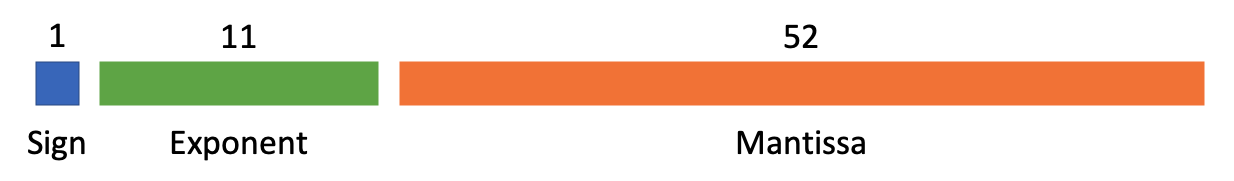
\includegraphics[width = 300pt]{Figure/fpu.png}
    \caption{A 64-bit Floating-Point Number}
    \label{fig:64bitfpr}
\end{figure}

The value is $(-1)^s \cdot 2^{e - 1023} \cdot \underbrace{(1 + \tilde{m} \cdot 2^{-52})}_{\times 2^{52} = m}$

For convenience, we may use $(s, e, m)$ to represent an FPN.

\end{frame}


\begin{frame}{Floating-Point Number Arithmetic}

\begin{columns}[T]
\column{0.5\textwidth}
FPN multiplication (FprMul) is proceeded by
    \only<2->{\begin{enumerate} \item Sign bit XOR}
    \only<3->{\item Exponent Addition}
    \only<4->{\item Mantissa Multiplication}
    \only<5->{\item Right-shifting the mantissa to $[2^{54}, 2^{55})$}
    \only<6->{\item Combining the results and rounding (FPR)}
\only<2->{\end{enumerate}}

\column{0.5\textwidth}
FPN addition (FprAdd) is proceeded by

    \only<7->{\begin{enumerate} \item  Making the first operand $\geq$ the second}
    \only<8->{ \item Right-shifting the second operand}
    \only<9->{ \item Mantissa Addition / Subtraction}
    \only<10->{ \item Normalizing the sum to $[2^{54}, 2^{55})$}
	\only<11->{\item  Combining the results and rounding (FPR)}
\only<7->{\end{enumerate}}

\end{columns}
\medskip

\pause

\end{frame}


\begin{frame}{Sticky Bit}

In floating-point arithmetic, when shifted right, the mantissa maintains a sticky bit
\[
1001\textcolor{black!50!green}{0}\textcolor{red}{0100} \gg 4 \to 1001\underbrace{\textcolor{blue}{1}}_{\text{Sticky}}
\]
It indicates whether there exists any $1$ after the least significant bit. In the above example,
\[
\text{sticky bit} = \textcolor{black!50!green}{0} \vee \llbracket (\textcolor{red}{0100}) \neq 0 \rrbracket = \llbracket (\textcolor{black!50!green}{0}\textcolor{red}{0100}) \neq 0 \rrbracket
\]

\end{frame}

\iffalse
%
%
%
%
%
%
\begin{frame}{Floating-Point Number Packing and Rounding}

\centerline{
\blockalgstart{.6\textwidth}{{\large FPR}}
\begin{algorithm}[H]
  \label{alg:FPR}
  \algsetup{linenosize=\small}
  \begin{algorithmic}[1]
    \REQUIRE Sign bit $s$, exponent $e$, and 55-bit mantissa $z$
    \ENSURE FPN $x$ packed by $s, e, z$
    \STATE $e \gets e + 1076$
    \STATE $b \gets \llbracket e < 0 \rrbracket$
    \STATE $z \gets z \wedge (b-1)$
    \STATE $b \gets \llbracket z \neq 0 \rrbracket $
    \STATE $e \gets e \wedge (-b)$
    \STATE $x \gets ((s \ll 63) \vee (z \gg 2)) + e \ll 52$
    \STATE $f \gets {\tt0XC8} \gg z^{[3:1]} $
    \STATE $x \gets x + f^{(1)}$ \COMMENT{increment if $z^{[3:1]}$ is 011,110 or 111} \\ 
    \RETURN \hskip -4pt $x$
  \end{algorithmic}
\end{algorithm}
\blockalgend
}

\end{frame}


\begin{frame}{Floating-Point Number Multiplication}

\centerline{
\blockalgstart{.9\textwidth}{{\large FprMul}}
\begin{algorithm}[H]
  \label{alg:fpr_mul}
  \algsetup{linenosize=\small}
  \begin{multicols}{2}
  \begin{algorithmic}[1]
    \REQUIRE FPN $x = (sx, ex, mx)$
    \REQUIRE FPN $y = (sy, ey, my)$
    \ENSURE FPN product of $x$ and $y$
    \STATE $s \gets sx \oplus sy$ \label{alg:FprMul:signbit}
    \STATE $e \gets ex + ey - 2100$ \label{alg:FprMul:exponent}
    \STATE $z \gets mx \times my$ \label{alg:FprMul:mantissa}
    \STATE $b \gets \llbracket z^{[50:1]} \neq 0 \rrbracket$
    \STATE $z \gets z^{[106:51]} \vee b$
    \STATE $z' \gets (z \gg 1) \vee z^{(1)}$
    \STATE $w \gets z^{(106)}$
    \STATE $z \gets z \oplus (z \oplus z') \wedge (-w)$
    \STATE $e \gets e + w$
    \STATE $bx \gets \llbracket ex \neq 0 \rrbracket$, $by \gets \llbracket ey \neq 0 \rrbracket$
    \STATE $b \gets bx \wedge by$
    \STATE $z \gets z \wedge (-b)$ \\
    \RETURN \hskip -4pt ${\sf FPR}(s, e, z)$
  \end{algorithmic}
  \end{multicols}
\end{algorithm}
\vspace{-10pt}
\blockalgend
}

\end{frame}


\begin{frame}{Floating-Point Number Addition}

\centerline{
\blockalgstart{.9\textwidth}{{\large FprAdd}}
\begin{algorithm}[H]
  \label{alg:fpr_add}
  \algsetup{linenosize=\small}
  \begin{multicols}{2}
  \small
  \begin{algorithmic}[1]
    \REQUIRE FPNs $x$ and $y$
    \ENSURE FPN sum of $x$ and $y$
    \STATE $d \gets x^{[63:1]} - y^{[63:1]}$
    \STATE $cs \gets d^{(64)} \vee ((1 - (-d)^{(64)}) \wedge x^{(64)}) $
    \STATE $m \gets (x \oplus y) \wedge (-cs)$
    \STATE $x \gets x \oplus m, y \gets y \oplus m$
    \STATE Extract $(sx, ex, mx)$ and $(sy, ey, my)$ from $x, y$, respectively.
    \STATE $mx \gets mx \ll 3, my \gets my \ll 3$
    \STATE $ex \gets ex - 1078, ey \gets ey - 1078$
    \STATE $c \gets ex - ey$
    \STATE $b \gets \llbracket c < 60 \rrbracket$ \label{alg:FprAdd:large_exp_start}
    \STATE $my \gets my \wedge (-b) $ \label{alg:FprAdd:large_exp_end}
    \STATE $my \gets (my \gg c) \vee \llbracket my^{[c:1]} \neq 0 \rrbracket$ \label{alg:FprAdd:unsigned-right-shift}
    \STATE $s \gets sx \oplus sy$
    \STATE $z \gets mx + (-1)^s my $
    \STATE Normalize $z, ex$ to make the 64th bit of $z$ set \label{alg:FprAdd:normalize}
    \STATE $z \gets (z \gg  9) \vee \llbracket z^{[9:1]} \neq 0 \rrbracket$
    \STATE $ex \gets ex + 9$ \\
    \RETURN \hskip -4pt ${\sf FPR}(sx, ex, z)$
  \end{algorithmic}
  \end{multicols}
\end{algorithm}
\vspace{-10pt}
\blockalgend
}

\end{frame}
%
%
%
%
\fi


\subsection{Power Analysis and Masking}
\begin{frame}{Power Analysis Attacks}

\begin{itemize}
\item Power consumption during the execution of programs depends on intermediate values.
\pause
\item Power analysis attacks leverage this fact to find the secret key. 
\pause
\end{itemize}
\vspace{-4pt}
\begin{figure}
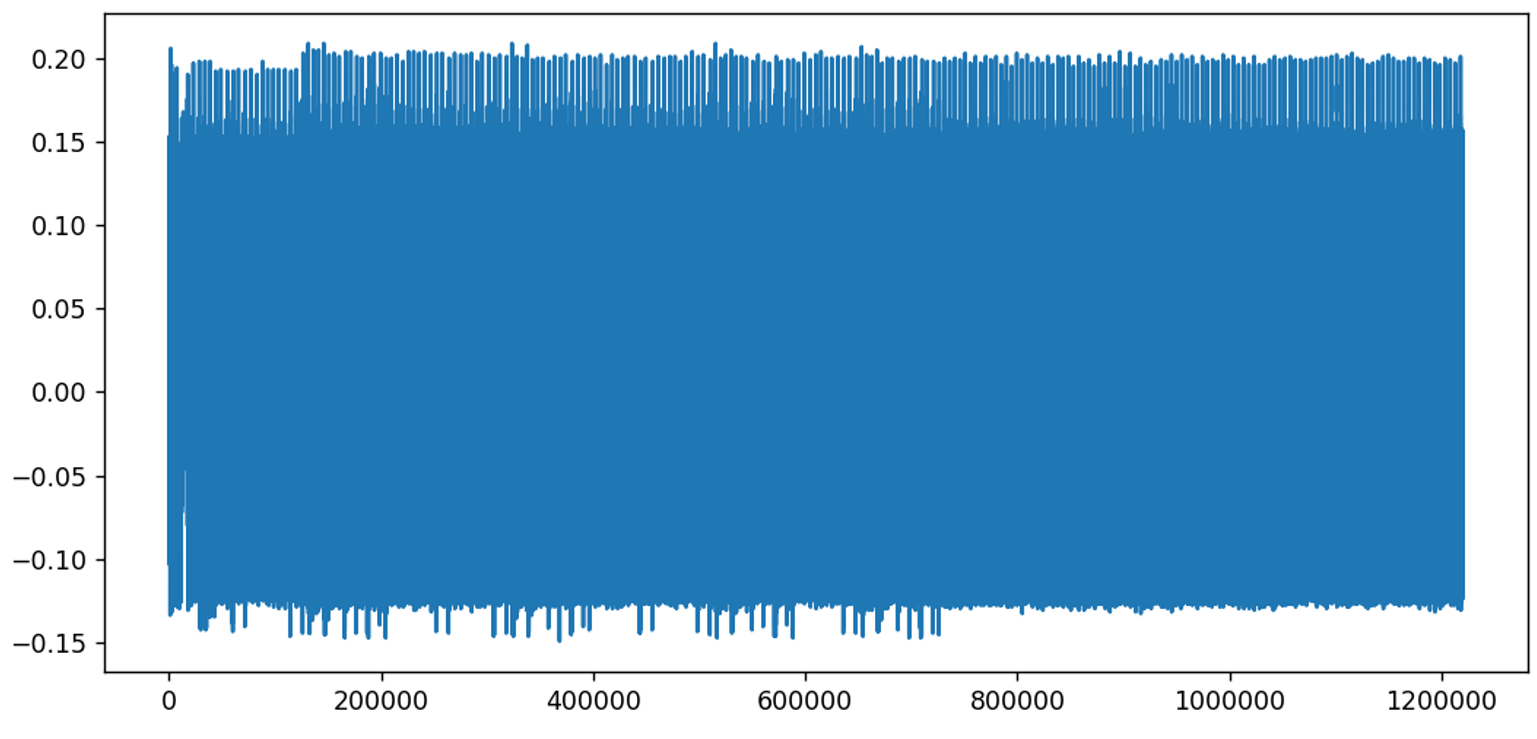
\includegraphics[width=.7\textwidth]{Figure/trace_example_ECC.png}
\vspace{-5pt}
\caption{An Example of a Power Trace}
\end{figure}

\end{frame}



\begin{frame}{Masking}

Masking defends against such threats by secret-sharing the sensitive variables.
\pause
\begin{itemize}
	\item Boolean Masking: A variable $x$ is split into $n$ shares $(x_i)_{1 \leq i \leq n}$ such that
	\[
	x = \bigoplus_{i=1}^n x_i
	\]
	\pause
	\item Arithmetic Masking: A variable $x$ is split into $n$ shares $(x_i)_{1 \leq i \leq n}$ (when stored in a $k$-bit register) such that
	\[
	x = \sum_{i=1}^n x_i \quad (\bmod\; 2^k)
	\]
\end{itemize}

\end{frame}


\begin{frame}{Masking}

\begin{itemize}
\item In each run, all $x_i$'s are randomized so that any $n-1$ shares of them are independently and uniformly distributed.
\pause
\item All operations need to be operated via shares.
\end{itemize}
\pause
For example, if $x$ is a secret variable, the operation $y \gets {\sf pt} \oplus x$ will become 
\[
	\begin{cases} y_1 \gets {\sf pt} \oplus x_1 \\ y_2 \gets x_2  \end{cases} \text{where } x_1,x_2 \getsdollar \{0,1\}^*, x_1 \oplus x_2 = x
\]

The variables with secret information are splitted into shares.

\end{frame}


%\begin{frame}{Probing Model}
%
%\begin{itemize}
%	\item The $t$-probing model \cite{C:IshSahWag03} assumes that an adversary is able to peek any $t$ intermediate values in the algorithm.
%	\item To be secure in $t$-probing model, $n \geq t+1$, and any share cannot be combined with each other.
%	\item It is complicated to prove $t$-probing security for a large composition of small algorithms (gadget). The concept of non-interference is convenient in this case.
%\end{itemize}
%
%\end{frame}
%
%
%
%\begin{frame}{Non-Interference Security}
%
%\begin{definition}{$t$-Non-Interference ($t$-NI) Security (from \cite{CCS:BBDFGS16})}
%A gadget is $t$-Non-Interference ($t$-NI) secure if every set of $t$ intermediate values can be simulated by no more than $t$ shares of each of its inputs.
%\end{definition}
%\medskip
%
%\begin{definition}{$t$-Strong Non-Interference ($t$-SNI) Security (from \cite{CCS:BBDFGS16})}
%A gadget is $t$-Strong-Non-Interference ($t$-SNI) secure if for every set of $t_I$ internal intermediate values and $t_O$ of its output shares with $t_I + t_O \leq t$, they can be simulated by no more than $t_I$ shares of each of its inputs.
%\end{definition}
%\medskip
%
%\end{frame}
%
%
%\begin{frame}{Non-Interference Security}
%
%In a nutshell,
%\begin{itemize}
%	\item $t$-SNI is stronger than $t$-NI by definition.
%	\item If a gadget is $t$-NI secure, and if any $n-1$ input shares are uniformly and independently distributed, then it is $t$-probing secure.
%	\item A composition of $t$-NI gadgets may not be $t$-NI, so we insert $t$-SNI gadgets to make it $t$-NI or $t$-SNI.
%\end{itemize}
%
%\end{frame}



\section{Masked Floating-Point Number Multiplication and Addition}

\subsection{Overview of Our Approach}
\begin{frame}{Overview of Our Approach}

We now show how we mask {\sf FPR}, {\sf FprMul}, and {\sf FprAdd}.
\pause

An intuitive approach to mask any algorithm:
\pause

\begin{itemize}
\item For operations like $\wedge, \oplus$: Boolean masking
\pause
\item For operations like $+, \times$: arithmetic masking
\end{itemize}
\pause
and use the following gadgets if necessary:
\pause
\begin{itemize}
	\item {\sf A2B}: $(x_i)_{1\leq i \leq n} \mapsto (y_i)_{1\leq i \leq n}$ such that $\sum_{i=1}^n x_i = \bigoplus_{i=1}^n y_i$
	\pause
	\item {\sf B2A}: $(y_i)_{1\leq i \leq n} \mapsto (x_i)_{1\leq i \leq n}$ such that $\bigoplus_{i=1}^n y_i = \sum_{i=1}^n x_i$
\end{itemize}

\end{frame}


\begin{frame}{Overview of Our Approach}

However, some operations in floating-point number arithmetic cannot be easily implemented in this way:
\pause
\begin{itemize}
	\item Checking whether a secret value is nonzero
	\begin{itemize}
		\item Given $(x_i)$, checking whether $\bigoplus_{i=1}^n x_i \neq 0$ or $\sum_{i=1}^n x_i \neq 0$
	\end{itemize}
	\pause
	\item Right-shifting a secret value by another secret value
	\begin{itemize}
		\item Given $(x_i)$ and $(c_i)$, right-shifting $(x_i)$ by $(c_i)$
	\end{itemize}
	\pause
	\item Normalizing a secret value to $[2^{63},2^{64})$
	\begin{itemize}
		\item Given $(x_i)$, left-shifting $(x_i)$ until its 64th bit is set
	\end{itemize}
\end{itemize}

\end{frame}

\iffalse
%
%
%
\begin{frame}{Overview of Our Approach}

%\only<2>{Checking whether a secret value is nonzero:}
%\only<3>{Right-shifting a secret value by another secret value:}
%\only<4>{Normalizing a secret value to $[2^{54},2^{55})$:}
%\medskip
Let's see where these operations are:
\begin{itemize}
	\item \alt<2>{\textcolor{red}{Checking whether a secret value is nonzero}} {Checking whether a secret value is nonzero}
	\item \alt<3>{\textcolor{red}{Right-shifting a secret value by another secret value}}{ Right-shifting a secret value by another secret value }
	\item \alt<4>{\textcolor{red}{Normalizing a secret value to $[2^{63},2^{64})$}}{Normalizing a secret value to $[2^{63},2^{64})$}
\end{itemize}


\begin{columns}[T]
\column{0.5\textwidth}
FprMul:
\begin{enumerate}
    \item {\color<2->{trans}{Sign bit XOR}}
    \item {\color<2->{trans}{Exponent Addition}}
    \item {\color<2->{trans}{Mantissa Multiplication}}
    \item \alt<1,3->{ {\color<3->{trans} Right-shifting the mantissa to $[2^{54}, 2^{55})$} }{ {\color{red}Right-shifting the mantissa to $[2^{54}, 2^{55})$} }
    \item \alt<1,3->{ {\color<3->{trans}Combining the results and rounding (FPR)} }{\color{red}Combining the results and rounding (FPR)}
\end{enumerate}

\column{0.5\textwidth}
FprAdd:
\begin{enumerate}
    \item {\color<2->{trans} Making the first operand $\geq$ the second}
    \item \alt<1,4->{ {\color<4->{trans} Right-shifting the second operand} }{ {\color{red} Right-shifting the second operand} }
    \item { \color<2->{trans}{Mantissa Addition / Subtraction} }
    \item \alt<1,3>{ {\color<3>{trans} Normalizing the sum to $[2^{54}, 2^{55})$} }{ {\color{red}Normalizing the sum to $[2^{54}, 2^{55})$} }
    \item \alt<1,3->{\color<3->{trans}Combining the results and rounding (FPR) }{\color{red}Combining the results and rounding (FPR)}
\end{enumerate}

\end{columns}
\medskip


\end{frame}
%
%
%
\fi



\begin{frame}{Overview of Our Approach}

We design novel gadgets for these three operations, including:
\pause
\begin{itemize}
	\item {\sf SecNonzero} (Algorithm \ref{alg:SecNonzero}): securely checking whether a secret value is nonzero.
	\pause
	\item {\sf SecFprUrsh} (Algorithm \ref{alg:SecFprUrsh}): securely right-shifting a secret value by another secret value
	\pause
	\item {\sf SecFprNorm64} (Algorithm \ref{alg:SecFprNorm64}): securely normalizing a secret value to $[2^{63}, 2^{64})$
\end{itemize}
\pause
In addition, we make several improvements to reduce the costs.

\end{frame}


\begin{frame}{Gadgets Used in Our Work}

\begin{table}
\centering
\begin{tabular}{ l l l} 
\toprule
\textbf{Gadget} & \textbf{Description} & \textbf{Reference} \\
\midrule
\sf SecAnd & AND of Boolean shares & \cite{C:IshSahWag03, CCS:BBDFGS16} \\
{\sf SecMult} & Multiplication of arithmetic shares & \cite{C:IshSahWag03, CCS:BBDFGS16} \\
{\sf SecAdd} & Addition of Boolean shares & \cite{FSE:CGTV15, EC:BBEFGR18} \\
{\sf A2B} & Arithmetic to Boolean conversion & \cite{PKC:SPOG19} \\
{\sf B2A} & Boolean to arithmetic conversion & \cite{TCHES:BetCorZei18} \\
${\sf B2A_{Bit}}$ & One-bit {\sf B2A} conversion & \cite{PKC:SPOG19} \\
{\sf RefreshMasks} & $t$-NI refresh of masks & \cite{CCS:BBDFGS16, TCHES:BetCorZei18} \\
{\sf Refresh} & $t$-SNI refresh of masks & \cite{CCS:BBDFGS16} \\
\bottomrule
\end{tabular}
\caption{List of used gadgets in our work}
\label{table:gadgets}
\end{table}

\end{frame}

\subsection{Tricks to Removing Branches}
\begin{frame}{Why Removing Branch}

\begin{itemize}
	\item For cryptographic operations, we need constant-time implementations.
	\pause
	\item Branch is usually not allowed in a constant-time implementation.
	\begin{itemize}
		\item Different operations can cause different running times (and power consumption patterns)
		\item Branch prediction
	\end{itemize}
\end{itemize}

\end{frame}

\begin{frame}{Tricks to Removing Branches}

If we want to run the following operations:
\centerline{
\blockalgstart{.2\textwidth}{}
\begin{algorithm}[H]
  \algsetup{linenosize=\small}
  \begin{algorithmic}[1]
    \IF{$a = 0$}
        \STATE $b \gets 0$
    \ENDIF
\end{algorithmic}
\end{algorithm}
\vspace{-2pt}
\blockalgend
}
\medskip
\pause

Suppose $a$ is either $0$ or $1$, we can write it as
\vskip -4pt
\centerline{
\blockalgstart{.2\textwidth}{}
\begin{algorithm}[H]
  \algsetup{linenosize=\small}
  \begin{algorithmic}[1]
    \STATE $b \gets b \wedge (-a)$
\end{algorithmic}
\end{algorithm}
\vspace{-3pt}
\blockalgend
}
\medskip
\pause

Now, for Boolean-shared values in our design
% \vskip -2pt
\centerline{
\blockalgstart{.34\textwidth}{}
\begin{algorithm}[H]
  \algsetup{linenosize=\small}
  \begin{algorithmic}[1]
    \STATE $(b_i) \gets {\sf SecAnd}((b_i), (-a_i))$
\end{algorithmic}
\end{algorithm}
\vspace{-3pt}
\blockalgend
}
\medskip

We utilize that $\bigoplus_{i=1}^n -a_i = -\bigoplus_{i=1}^n a_i = -a$, which is not true for a general $k$-bit $a$.
\end{frame}


\begin{frame}{Tricks to Removing Branches}

Similarly, for operations
\centerline{
\blockalgstart{.2\textwidth}{}
\begin{algorithm}[H]
  \algsetup{linenosize=\small}
  \begin{algorithmic}[1]
    \IF{$a = 1$}
        \STATE $b \gets 0$
    \ENDIF
\end{algorithmic}
\end{algorithm}
\vspace{-2pt}
\blockalgend
}
\medskip
\pause

Suppose $a$ is either $0$ or $1$, we can write it as
\vskip -4pt
\centerline{
\blockalgstart{.23\textwidth}{}
\begin{algorithm}[H]
  \algsetup{linenosize=\small}
  \begin{algorithmic}[1]
    \STATE $b \gets b \wedge (\neg(-a))$
\end{algorithmic}
\end{algorithm}
\vspace{-3pt}
\blockalgend
}
\medskip
\pause

For Boolean-shared values,
% \vskip -2pt
\centerline{
\blockalgstart{.45\textwidth}{}
\begin{algorithm}[H]
  \algsetup{linenosize=\small}
  \begin{algorithmic}[1]
    \STATE $(c_i) \gets (-a_i)$
    \STATE $(b_i) \gets {\sf SecAnd}((b_i), (\neg c_1, c_2, \cdots, c_n))$
\end{algorithmic}
\end{algorithm}
\vspace{-3pt}
\blockalgend
}
\medskip

We utilize that $\neg \left( \bigoplus_{i=1}^n c_i \right) = (\neg c_1) \oplus \left( \bigoplus_{i=2}^n c_i \right)$.
\end{frame}


\begin{frame}{Tricks to Removing Branches}

Moreover, for operations,
\centerline{
\blockalgstart{.2\textwidth}{}
\begin{algorithm}[H]
  \algsetup{linenosize=\small}
  \begin{algorithmic}[1]
    \IF{$a = 1$}
        \STATE $b \gets c$
    \ENDIF
\end{algorithmic}
\end{algorithm}
\vspace{-2pt}
\blockalgend
}
\medskip
\pause

Suppose $a$ is either $0$ or $1$, we may write it as
\vskip -4pt
\centerline{
\blockalgstart{.25\textwidth}{}
\begin{algorithm}[H]
  \algsetup{linenosize=\small}
  \begin{algorithmic}[1]
    \STATE $d \gets b \oplus c$
    \STATE $b \gets b \oplus (d \wedge (-a))$
\end{algorithmic}
\end{algorithm}
\vspace{-3pt}
\blockalgend
}
\medskip
\pause

For Boolean-shared values,
% \vskip -2pt
\centerline{
\blockalgstart{.35\textwidth}{}
\begin{algorithm}[H]
  \algsetup{linenosize=\small}
  \begin{algorithmic}[1]
    \STATE $(d_i) \gets (b_i \oplus c_i)$
    \STATE $(d_i) \gets {\sf SecAnd}((d_i), (-a_i))$
    \STATE $(b_i) \gets (b_i \oplus d_i)$
\end{algorithmic}
\end{algorithm}
\vspace{-3pt}
\blockalgend
}
\medskip
\end{frame}



\begin{frame}{Tricks in Masking FPR}

\centerline{
\blockalgstart{.6\textwidth}{{\large FPR}}
\begin{algorithm}[H]
  \algsetup{linenosize=\small}
  \begin{algorithmic}[1]
    \REQUIRE Sign bit $s$, exponent $e$, and 55-bit mantissa $z$
    \ENSURE FPN $x$ packed by $s, e, z$
    \STATE $e \gets e + 1076$
    \STATE $b \gets \llbracket e < 0 \rrbracket$
    \STATE \textcolor{red}{$z \gets z \wedge (b-1)$}
    \STATE $b \gets \llbracket z \neq 0 \rrbracket $
    \STATE \textcolor{red}{$e \gets e \wedge (-b)$}
    \STATE $x \gets ((s \ll 63) \vee (z \gg 2)) + e \ll 52$
    \STATE $f \gets {\tt0XC8} \gg z^{[3:1]} $
    \STATE $x \gets x + f^{(1)}$ \COMMENT{increment if $z^{[3:1]}$ is 011,110 or 111} \\ 
    \RETURN \hskip -4pt $x$
  \end{algorithmic}
\end{algorithm}
\blockalgend
}

\end{frame}


\begin{frame}{Tricks in Masking FprMul}

\centerline{
\blockalgstart{.9\textwidth}{{\large FprMul}}
\begin{algorithm}[H]
  \algsetup{linenosize=\small}
  \begin{multicols}{2}
  \begin{algorithmic}[1]
    \REQUIRE FPN $x = (sx, ex, mx)$
    \REQUIRE FPN $y = (sy, ey, my)$
    \ENSURE FPN product of $x$ and $y$
    \STATE $s \gets sx \oplus sy$ 
    \STATE $e \gets ex + ey - 2100$ 
    \STATE $z \gets mx \times my$
    \STATE $b \gets \llbracket z^{[50:1]} \neq 0 \rrbracket$
    \STATE $z \gets z^{[106:51]} \vee b$
    \STATE $z' \gets (z \gg 1) \vee z^{(1)}$
    \STATE $w \gets z^{(106)}$
    \STATE \textcolor{red}{$z \gets z \oplus (z \oplus z') \wedge (-w)$}
    \STATE $e \gets e + w$
    \STATE $bx \gets \llbracket ex \neq 0 \rrbracket$, $by \gets \llbracket ey \neq 0 \rrbracket$
    \STATE $b \gets bx \wedge by$
    \STATE \textcolor{red}{$z \gets z \wedge (-b)$} \\
    \RETURN \hskip -4pt ${\sf FPR}(s, e, z)$
  \end{algorithmic}
  \end{multicols}
\end{algorithm}
\vspace{-10pt}
\blockalgend
}

\end{frame}


\begin{frame}{Tricks in Masking FprAdd}

\centerline{
\blockalgstart{.9\textwidth}{{\large FprAdd}}
\begin{algorithm}[H]
  \algsetup{linenosize=\small}
  \begin{multicols}{2}
  \small
  \begin{algorithmic}[1]
    \REQUIRE FPNs $x$ and $y$
    \ENSURE FPN sum of $x$ and $y$
    \STATE $d \gets x^{[63:1]} - y^{[63:1]}$
    \STATE $cs \gets d^{(64)} \vee ((1 - (-d)^{(64)}) \wedge x^{(64)}) $
    \STATE \textcolor{red}{$m \gets (x \oplus y) \wedge (-cs)$}
    \STATE \textcolor{red}{$x \gets x \oplus m, y \gets y \oplus m$}
    \STATE Extract $(sx, ex, mx)$ and $(sy, ey, my)$ from $x, y$, respectively.
    \STATE $mx \gets mx \ll 3, my \gets my \ll 3$
    \STATE $ex \gets ex - 1078, ey \gets ey - 1078$
    \STATE $c \gets ex - ey$
    \STATE $b \gets \llbracket c < 60 \rrbracket$ 
    \STATE \textcolor{red}{$my \gets my \wedge (-b) $ }
    \STATE $my \gets (my \gg c) \vee \llbracket my^{[c:1]} \neq 0 \rrbracket$
    \STATE $s \gets sx \oplus sy$
    \STATE $z \gets mx + (-1)^s my $
    \STATE Normalize $z, ex$ to make the 64th bit of $z$ set
    \STATE $z \gets (z \gg  9) \vee \llbracket z^{[9:1]} \neq 0 \rrbracket$
    \STATE $ex \gets ex + 9$ \\
    \RETURN \hskip -4pt ${\sf FPR}(sx, ex, z)$
  \end{algorithmic}
  \end{multicols}
\end{algorithm}
\vspace{-10pt}
\blockalgend
}

\end{frame}



\subsection*{Wrapping-up}
\begin{frame}{Wrapping-up}

Utilizing these new gadgets {\sf SecNonzero}, {\sf SecFprUrsh}, and {\sf SecFprNorm64}, we design the following algorithms:
\pause
\begin{itemize}
	\item {\sf SecFPR}: Secure FPR by masking.
	\pause
	\item {\sf SecFprMul}: Secure FprMul by masking.
	\pause
	\item {\sf SecFprAdd}: Secure FprAdd by masking.
\end{itemize}
\pause
We leave the details of the implementations and several tricks for improvements in \hyperlink{sec:appendix}{Appendix}.

\end{frame}
%\begin{frame}{SecFPR: Secure FPR}

\begin{columns}[T]
\column{.6\textwidth}
\begin{block}{{\large FPR}}
\begin{algorithm}[H]
  \algsetup{linenosize=\small}
  \begin{algorithmic}[1]
    \REQUIRE \textcolor<2>{red}{ Sign bit $s$, exponent $e$, and 55-bit mantissa $z$}
    \ENSURE FPN $x$ packed by $s, e, z$
    \STATE \textcolor<3>{red}{$e \gets e + 1076$}

    \STATE \textcolor<4>{red}{$b \gets \llbracket e < 0 \rrbracket$}

    \STATE \textcolor<4>{red}{$z \gets z \wedge (b-1)$}
   
    \STATE \textcolor<5>{red}{$b \gets \llbracket z \neq 0 \rrbracket $}

    \STATE \textcolor<6>{red}{ $e \gets e \wedge (-b)$ }

    \STATE \textcolor<6>{red}{ $x \gets ((s \ll 63) \vee (z \gg 2)) + e \ll 52$}

    \STATE \textcolor<7>{red}{$f \gets {\tt0XC8} \gg z^{[3:1]} $ }

    \STATE \textcolor<7>{red}{$x \gets x + f^{(1)}$} \\ 
    \RETURN \hskip -12pt \textcolor<8>{red}{$x$}
  \end{algorithmic}
\end{algorithm}
\end{block}

\column{.35\textwidth}


\only<1>{
\vskip 70pt
We now show how we mask the floating-point number rounding and packing algorithm {\sf FPR}.
}


\only<2>{
\vskip 50pt
Recall that {\sf FPR} is the last subroutine of {\sf FprMul} and {\sf FprAdd}.

By our masking design of {\sf FprMul} and {\sf FprAdd}, $(s_i)$ is Boolean-masked, $(e_i)$ is 16-bit arithmetic-masked, and $(z_i)$ is Boolean-masked.
}


\only<3>{
\vskip 70pt
This is by adding to any one share.
}


\only<4>{
\vskip 50pt
This is equivalent to
\centerline{
\blockalgstart{.6\textwidth}{}
\begin{algorithm}[H]
  \algsetup{linenosize=\small}
  \begin{algorithmic}[1]
    \IF{$e < 0$}
        \STATE $z \gets 0$
    \ENDIF
\end{algorithmic}
\end{algorithm}
\blockalgend
}

\medskip
and is done by an ${\sf A2B}$, taking the MSB, and the simple trick.
}


\only<5>{
\vskip 70pt
This is done by {\sf SecNonzero} and the simple trick.
}


\only<6>{
\vskip 50pt
Shift, OR, and a {\sf SecAdd}.

We add $(e_i)$ and the $55$th bit of $(z_i)$ in advance instead of adding $(e_i)$ to a 64-bit value. That is, use a 16-bit {\sf SecAdd} to save a 64-bit {\sf SecAdd} 
}


\only<7>{
\vskip 50pt
If the least 3 bits of $(z_i)$ are 011, 110, and 111, $f^{(1)} = 1$.

We OR $(z^{(1)}_i)$ and $(z^{(3)}_i)$ by {\sf SecOr}, and then AND $(z^{(2)}_i)$ by {\sf SecAnd}. The result is then added to $(x_i)$ by {\sf SecAdd}.
}


\only<8>{
\vskip 70pt
Done.

The returned value is a 64-bit Boolean-masked $(x_i)$.
}

\end{columns}

\end{frame}



\begin{frame}{SecFPR: Secure FPR}

\centerline{
\blockalgstart{\textwidth}{{\large SecFPR}}
\begin{algorithm}[H]
  \algsetup{linenosize=\small}
  \label{alg:SecFPR}
  \begin{multicols}{2}
  \begin{algorithmic}[1]
    \REQUIRE 1-bit Boolean shares ${(s_i)_{1\leq i \leq n}}$
	\REQUIRE 16-bit arithmetic shares ${(e_i)_{1\leq i \leq n}}$
	\REQUIRE 55-bit Boolean shares ${(z_i)_{1\leq i \leq n}}$
    \ENSURE Boolean shares ${(x_i)_{1\leq i \leq n}}$
    \STATE $e_1 \gets e_1 + 1076$
    \STATE $(e_i) \gets {\sf A2B}( (e_i) )$ \label{alg:SecFPR:A2B}
    \STATE $(b_i) \gets (-e_i^{(16)})$
    \STATE $(z_i) \gets {\sf SecAnd}( (z_i), {(\neg b_1, b_2, \cdots, b_n)} )$\label{alg:SecFPR:comp}
    % \STATE $(b_i) \gets ( -z_i^{(55)} )$
    \STATE $(e_i) \gets {\sf SecAnd}( (e_i), {(-z_i^{(55)})} )$\label{alg:SecFPR:zero}
    \STATE $(e_i) \gets {\sf SecAdd}( (e_i), (z_i^{(55)}) )$ \label{alg:SecFPR:SecAdd_1}
    \STATE $(e_i) \gets {\sf Refresh}((e_i))$
    \STATE $(s_i) \gets {\sf Refresh}((s_i))$
    \STATE $(x_i) \gets ((s_i^{(1)} \ll 63) \vee (e_i^{[11:1]} \ll 52 ) \; \vee (z_i^{[54:3]})$ \label{alg:SecFPR:pack}
    \STATE $(f_i) \gets {\sf SecOr}( {\sf Refresh}(z_i^{(1)}) , (z_i^{(3)}))$ \label{alg:SecFPR:OR}
    \STATE $(f_i) \gets {\sf SecAnd}((f_i) , (z_i^{(2)}))$ \label{alg:SecFPR:AND}
    \STATE $(x_i) \gets {\sf SecAdd}( (x_i), (f_i) )$ \label{alg:SecFPR:SecAdd_2}
    \STATE \Return $(x_i)$
  \end{algorithmic}
  \end{multicols}
   \vskip -10pt
\end{algorithm}
\blockalgend
}


\end{frame}
%\ifhandout
\else

\begin{frame}{SecFprMul: Secure FprMul}

\centerline{
\blockalgstart{.9\textwidth}{{\large FprMul}}
\begin{algorithm}[H]
  \algsetup{linenosize=\small}
  \begin{multicols}{2}
  \begin{algorithmic}[1]
    \REQUIRE \textcolor<2>{red}{FPN $x = (sx, ex, mx)$}
    \REQUIRE \textcolor<2>{red}{FPN $y = (sy, ey, my)$}
    \ENSURE FPN product of $x$ and $y$

    \STATE \textcolor<3>{red}{ $s \gets sx \oplus sy$}
    \STATE \textcolor<3>{red}{ $e \gets ex + ey - 2100$}

    \STATE \textcolor<4>{red}{$z \gets mx \times my$}

    \STATE \textcolor<5-6>{red}{ $b \gets \llbracket z^{[50:1]} \neq 0 \rrbracket$}
    \STATE \textcolor<5-6>{red}{ $z \gets z^{[106:51]} \vee b$ }
    \STATE \textcolor<5-6>{red}{ $z' \gets (z \gg 1) \vee z^{(1)}$ }
    \STATE \textcolor<5-6>{red}{ $w \gets z^{(106)}$ }
    \STATE \textcolor<5-6>{red}{$z \gets z \oplus (z \oplus z') \wedge (-w)$ }

    \STATE \textcolor<7>{red}{$e \gets e + w$}
 
    \STATE \textcolor<8>{red}{$bx \gets \llbracket ex \neq 0 \rrbracket$, $by \gets \llbracket ey \neq 0 \rrbracket$}
    \STATE \textcolor<8>{red}{$b \gets bx \wedge by$}
    \STATE \textcolor<8>{red}{$z \gets z \wedge (-b)$} \\
    \RETURN \hskip -4pt \textcolor<9>{red}{${\sf FPR}(s, e, z)$}
  \end{algorithmic}
  \end{multicols}
\vspace{-10pt}
\end{algorithm}

\blockalgend
}
\medskip

\only<1>{
We show how we mask the floating-point number multiplication algorithm {\sf FprMul}.
}

\only<2>{
We assume $(sx_i)$ and $(sy_i)$ are Boolean shares, $(ex_i)$ and $(ey_i)$ are 16-bit arithmetic shares, and $(mx_i)$ and $(my_i)$ are 128-bit arithmetic shares, which can load the product of two $53$-bit values.
}


\only<3>{
These can be operated share-wise.
}


\only<4>{
This is done by {\sf SecMult}. For further operations, we then apply an {\sf A2B} to turn them to Boolean shares.
}


\only<5>{
Conditional shift by $50$ bits and $51$ bits, depending on $z^{(106)}$, while preserving the sticky bit.

These can be done by {\sf SecNonzero} and {\sf SecOr}.

}

\only<6>{
We observe that we can save one {\sf SecOr}.
\begin{itemize}
\item When shifted by $50$ bits, we OR the last bit with $z^{[50:1]}$.
\item When shifted by $51$ bits, we OR the last bit with $z^{[51:1]}$.
\end{itemize}
We can simply OR the the last bit with $z^{[51:1]}$, regardless of the conditional shift result.
}


\only<7>{
This is by adding to any share.
}



\only<8>{
This is by {\sf SecNonzero} and {\sf SecAnd}, and applying the tricks.
}



\only<9>{
Now it calls {\sf FPR} to return a 64-bit Boolean-masked FPN.
}

\end{frame}

%
%
%
\fi


\begin{frame}{SecFprMul: Secure FprMul}


\centerline{
\blockalgstart{\textwidth}{SecFprMul}
\begin{algorithm}[H]
  \algsetup{linenosize=\small}
  \label{alg:SecFprMul}
  \small
  \begin{multicols}{2}
  \begin{algorithmic}[1]
    \REQUIRE Shares ${(sx_i)_{1\leq i \leq n}}, {(ex_i)_{1\leq i \leq n}}, {(mx_i)_{1\leq i \leq n}}$
    \REQUIRE Shares ${(sy_i)_{1\leq i \leq n}}, {(ey_i)_{1\leq i \leq n}}, {(my_i)_{1\leq i \leq n}}$
    \ENSURE Boolean shares for the FPN product.
    \STATE $(s_i) \gets (sx_i \oplus sy_i)$ \label{alg:SecFprMul:sign_add}
    \STATE $(e_i) \gets (ex_1 + ey_1 - 2100, ex_2 + ey_2, \cdots)$ \label{alg:SecFprMul:exp_add}
    \STATE $(p_i) \gets {\sf SecMult}((mx_i), (my_i))$ \label{alg:SecFprMul:mant_mul}
    \STATE $(p_i) \gets {\sf A2B}((p_i))$ \label{alg:SecFprMul:128A2B}
    \STATE $(b_i) \gets {\sf SecNonzero}( (p_i^{[51:1]}) )$ \label{alg:SecFprMul:bool_nonzero}
    \STATE $(z_i) \gets (p_i^{[105:51]})$ \label{alg:SecFprMul:shift_start}
    \STATE $(z'_i) \gets (p_i^{[105:51]} \oplus p_i^{[106:52]})$
    \STATE $(w_i) \gets (p_i^{(106)})$
    \STATE $(z'_i) \gets {\sf SecAnd}( (z'_i), {\sf Refresh}((-w_i) ))$ \label{alg:SecFprMul:condition}
    \STATE $(z_i) \gets (z'_i \oplus z_i)$ \label{alg:SecFprMul:shift}
    \STATE $(z_i) \gets {\sf SecOr}( (z_i), (b_i) )$ \label{alg:SecFprMul:stickybit}
    \STATE $(w_i) \gets {\sf B2A_{Bit}}((w_i))$
    \STATE $(e_i) \gets (e_i + w_i)$ \label{alg:SecFprMul:add106}
    \STATE $(bx_i) \gets {\sf SecNonzero}( (ex_i) )$ \label{alg:SecFprMul:arith_nonzero_1}
    \STATE $(by_i) \gets {\sf SecNonzero}( (ey_i) )$ \label{alg:SecFprMul:arith_nonzero_2}
    \STATE $(d_i) \gets {\sf SecAnd}( (bx_i), (by_i) )$
    \STATE $(z_i) \gets {\sf SecAnd}( (z_i) , (-d_i^{(1)}) )$ \label{alg:SecFprMul:check_exp}
    \STATE \Return ${\sf SecFPR}( (s_i) , (e_i) , (z_i) )$
  \end{algorithmic}
  \end{multicols}
\vspace{-10pt}
\end{algorithm}

\blockalgend
}
\medskip



\end{frame}



\section{Evaluation and Implementation}

\subsection{Security}
\begin{frame}{Probing Model}

To theoretically evaluate the security of our design, we consider the probing model \cite{C:IshSahWag03}.
\pause
\begin{itemize}
	\item The $t$-probing model assumes that an adversary is able to peek any $t$ intermediate values in the algorithm.
	\pause
	\item To be secure in $t$-probing model, $n \geq t+1$, and any share cannot be combined with each other.
	\pause
	\item It is complicated to prove $t$-probing security for a large composition of small gadgets. The concept of non-interference is convenient in this case.
\end{itemize}

\end{frame}


\begin{frame}{Non-Interference Security}

\begin{definition}{$t$-Non-Interference ($t$-NI) Security (from \cite{CCS:BBDFGS16})}
A gadget is $t$-Non-Interference ($t$-NI) secure if every set of $t$ intermediate values can be simulated by no more than $t$ shares of each of its inputs.
\end{definition}
\medskip

\begin{definition}{$t$-Strong Non-Interference ($t$-SNI) Security (from \cite{CCS:BBDFGS16})}
A gadget is $t$-Strong-Non-Interference ($t$-SNI) secure if for every set of $t_I$ internal intermediate values and $t_O$ of its output shares with $t_I + t_O \leq t$, they can be simulated by no more than $t_I$ shares of each of its inputs.
\end{definition}
\medskip

\end{frame}


\begin{frame}{Non-Interference Security}

For $t = n-1$, if a gadget is $t$-NI or $t$-SNI secure, and if any $n-1$ input shares are uniformly and independently distributed, then it is $t$-probing secure.
\medskip

\pause
Moreover,
\pause
\begin{itemize}
	\item $t$-SNI is stronger than $t$-NI by definition.
	\pause
	\item A composition of $t$-NI gadgets may not be $t$-NI, so we insert $t$-SNI gadgets to make it $t$-NI or $t$-SNI.
\end{itemize}
\pause
All the gadgets/algorithms in our paper are proven either $t$-NI or $t$-SNI secure.

\end{frame}


\begin{frame}{Gadgets/Algorithms in Our Work}

\begin{table}
\centering
\begin{tabular}{l l | l l} 
\toprule
\textbf{Algorithm} & \textbf{Security$\quad$} & \textbf{Algorithm} & \textbf{Security$\quad$} \\
\midrule
{\sf SecAnd} & $t$-SNI & {\sf SecOr} & $t$-SNI \\
{\sf SecMult} & $t$-SNI & {\sf SecNonzero} & $t$-SNI \\
{\sf SecAdd} & $t$-NI & {\sf SecFprUrsh} & $t$-SNI \\
{\sf A2B} & $t$-SNI & {\sf SecFprNorm64} & $t$-NI\\
{\sf B2A} & $t$-SNI & {\sf SecFPR} & $t$-SNI \\
${\sf B2A_{Bit}}$ & $t$-SNI & {\sf SecFprMul} & $t$-SNI\\
{\sf RefreshMasks} & $t$-NI & {\sf SecFprAdd} & $t$-SNI\\
{\sf Refresh} & $t$-SNI \\
\bottomrule
\end{tabular}
\caption{List of gadgets/algorithms in our work with $n=t+1$ shares}
\label{table:gadgets_secureity}
\end{table}
\end{frame}

\begin{frame}{Test Vector Leakage Assessment (TVLA)}

Probing model validates the security theoretically.
\pause

In practice, the Test Vector Leakage Assessment (TVLA) methodology \cite{gilbert2011testing} can be applied.
\pause

A tester records two sets of traces where
\pause

\begin{itemize}
	\item Set 1: fixed input
	\pause
	\item Set 2: random input
\end{itemize}
\pause

The Welch's $t$-test is then applied on the two sets.
\pause

By convention, we consider the leakage is significant if the $t$-value exceeds $\pm 4.5$.
\pause

For traces with a large number of points, we refer to \cite{ding2018towards} alter this threshold to avoid false positives.

\end{frame}


\begin{frame}{Experiment Setup}

We implement our algorithms in the following setting:
\pause

\begin{itemize}
\item Plain-C code
\pause
\item Compiled by {\tt arm-none-eabi-gcc 10.3.1}
\pause
\item Using ChipWhisperer with target board STM32F303 with an Arm Cortex-M4 MCU
\pause
\item We compare the result with the reference implementation of the NIST Round-3 Submission of \textsc{Falcon} \cite{NISTPQC-R3:FALCON20}.
\end{itemize}

\end{frame}




\begin{frame}{TVLA}

The TVLA results of floating-point number multiplication (FprMul, SecFprMul).

\begin{columns}[T]
\column{.34\textwidth}
\begin{figure}
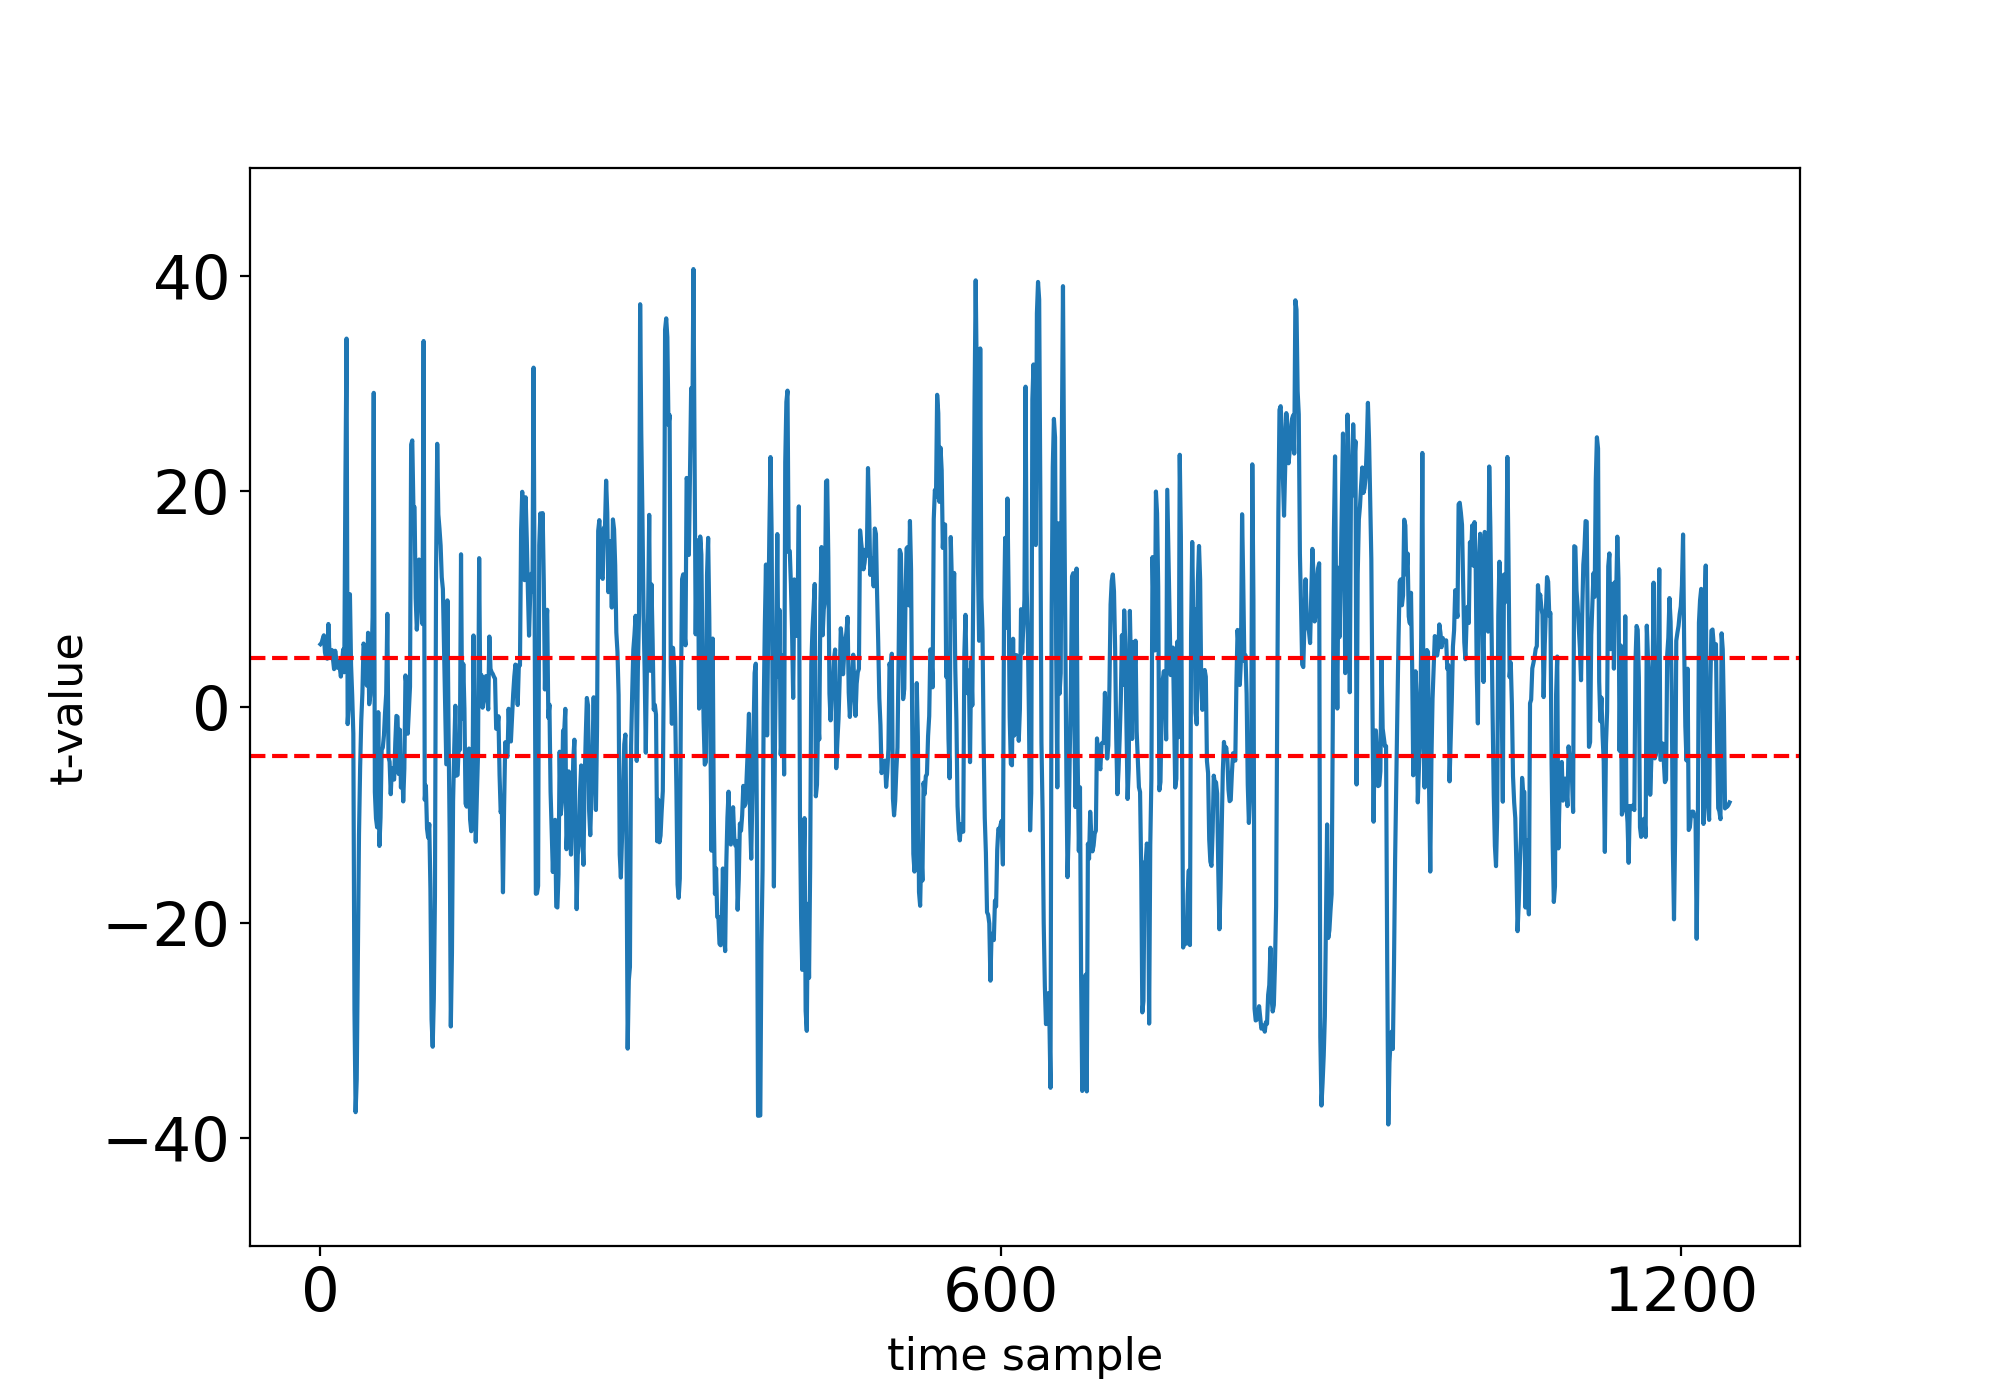
\includegraphics[width=\textwidth]{Figure/tvla/fprmul_1k.png}
\vspace{-20pt}
\caption{1,000 traces, unmasked FprMul}
\end{figure}

\column{.34\textwidth}
\begin{figure}
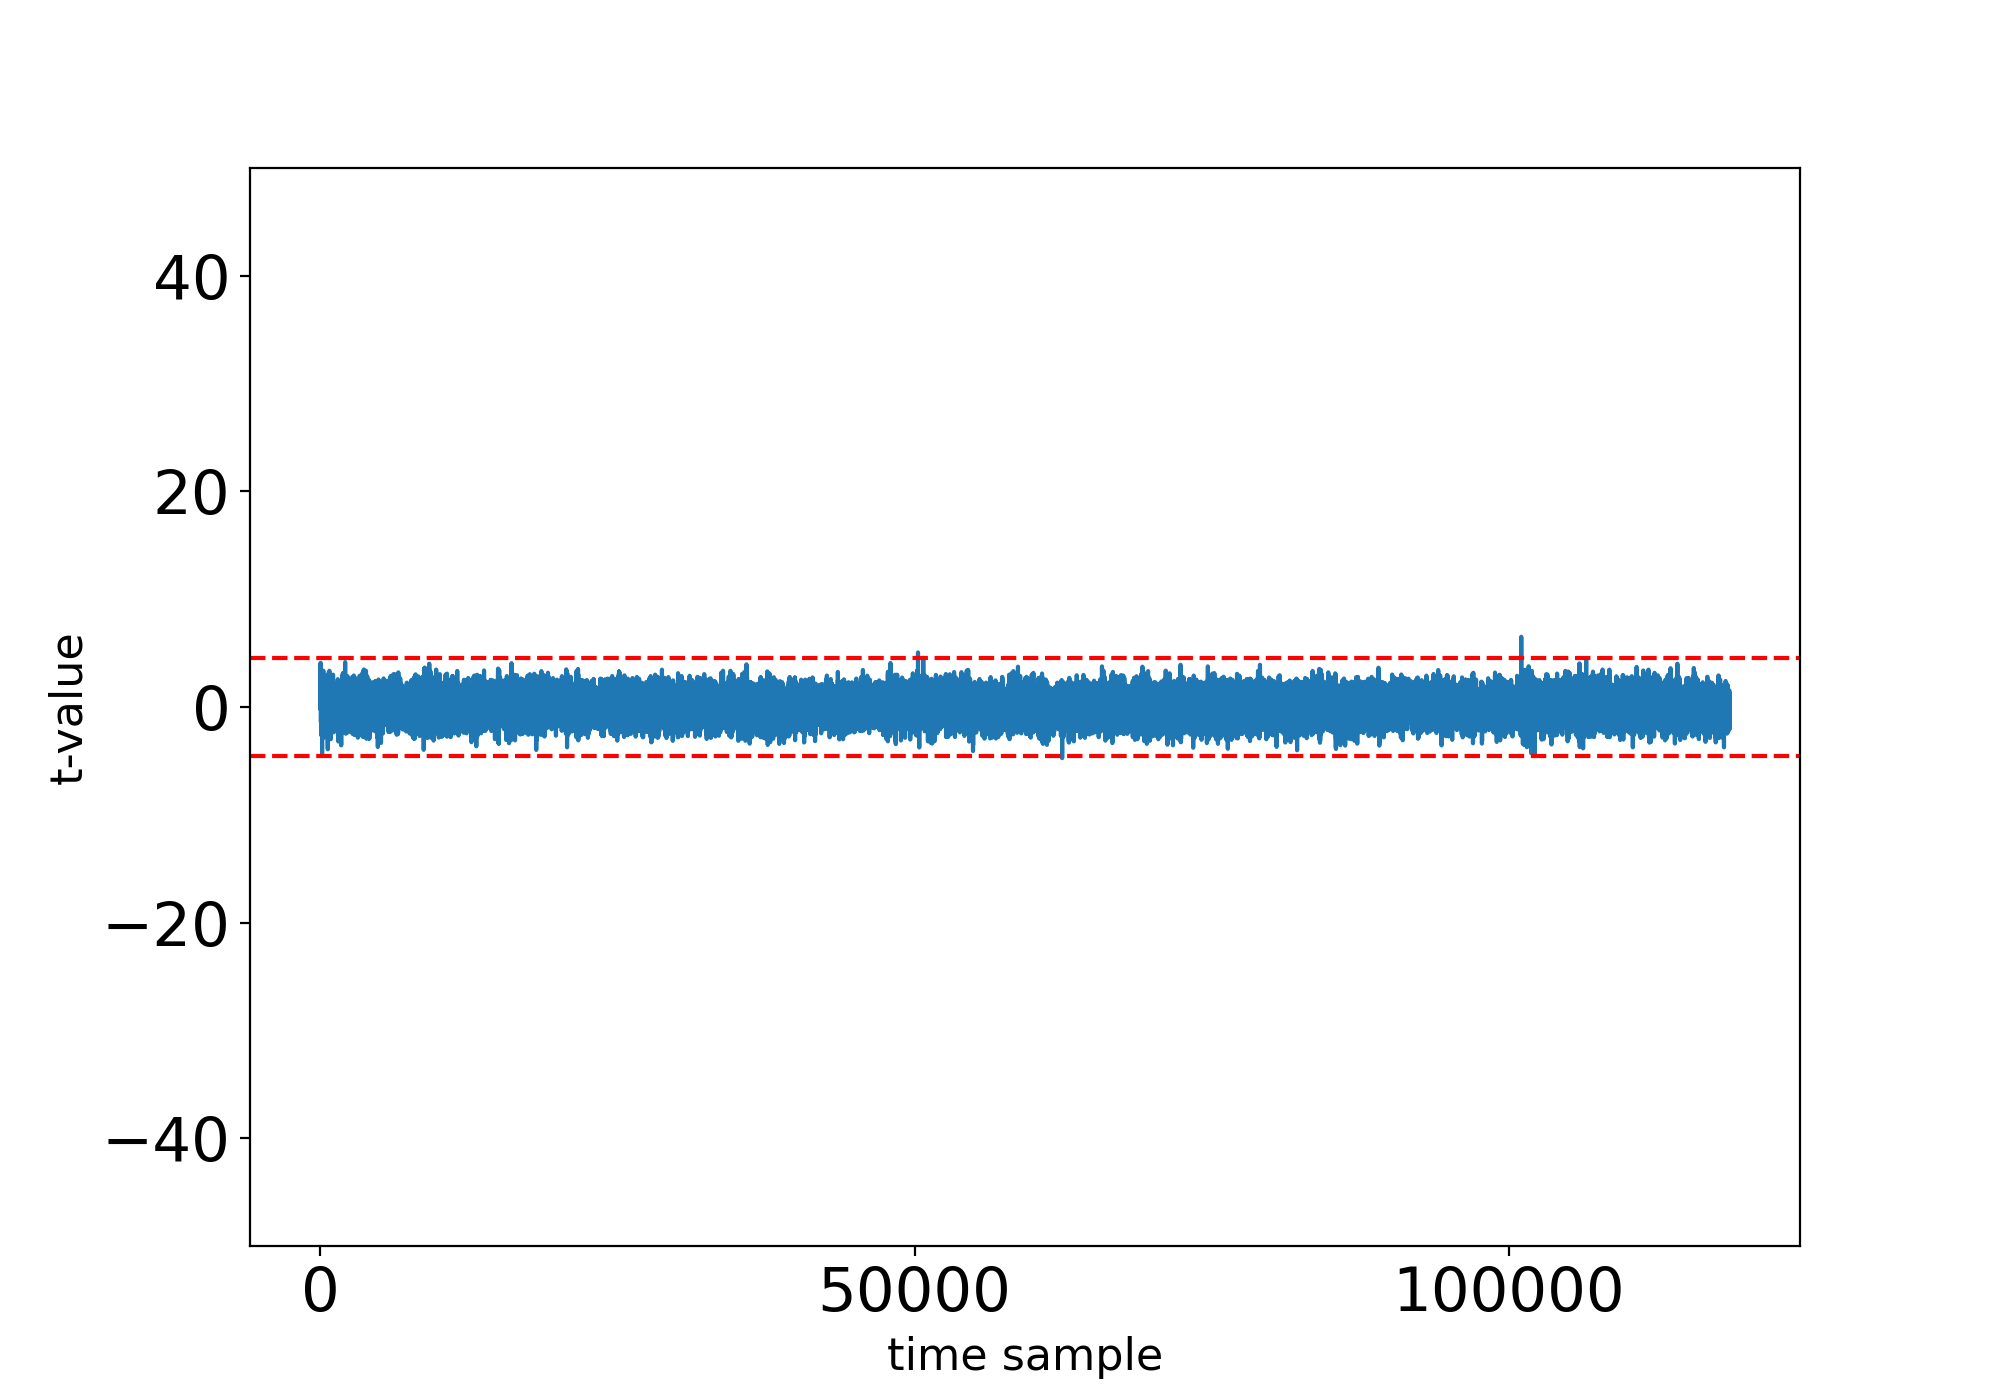
\includegraphics[width=\textwidth]{figure/tvla/1013_SecFprMul_2shares_10k.png}
\vspace{-20pt}
\caption{10,000 traces, 2-shared SecFprMul}
\end{figure}

\column{.34\textwidth}
\begin{figure}
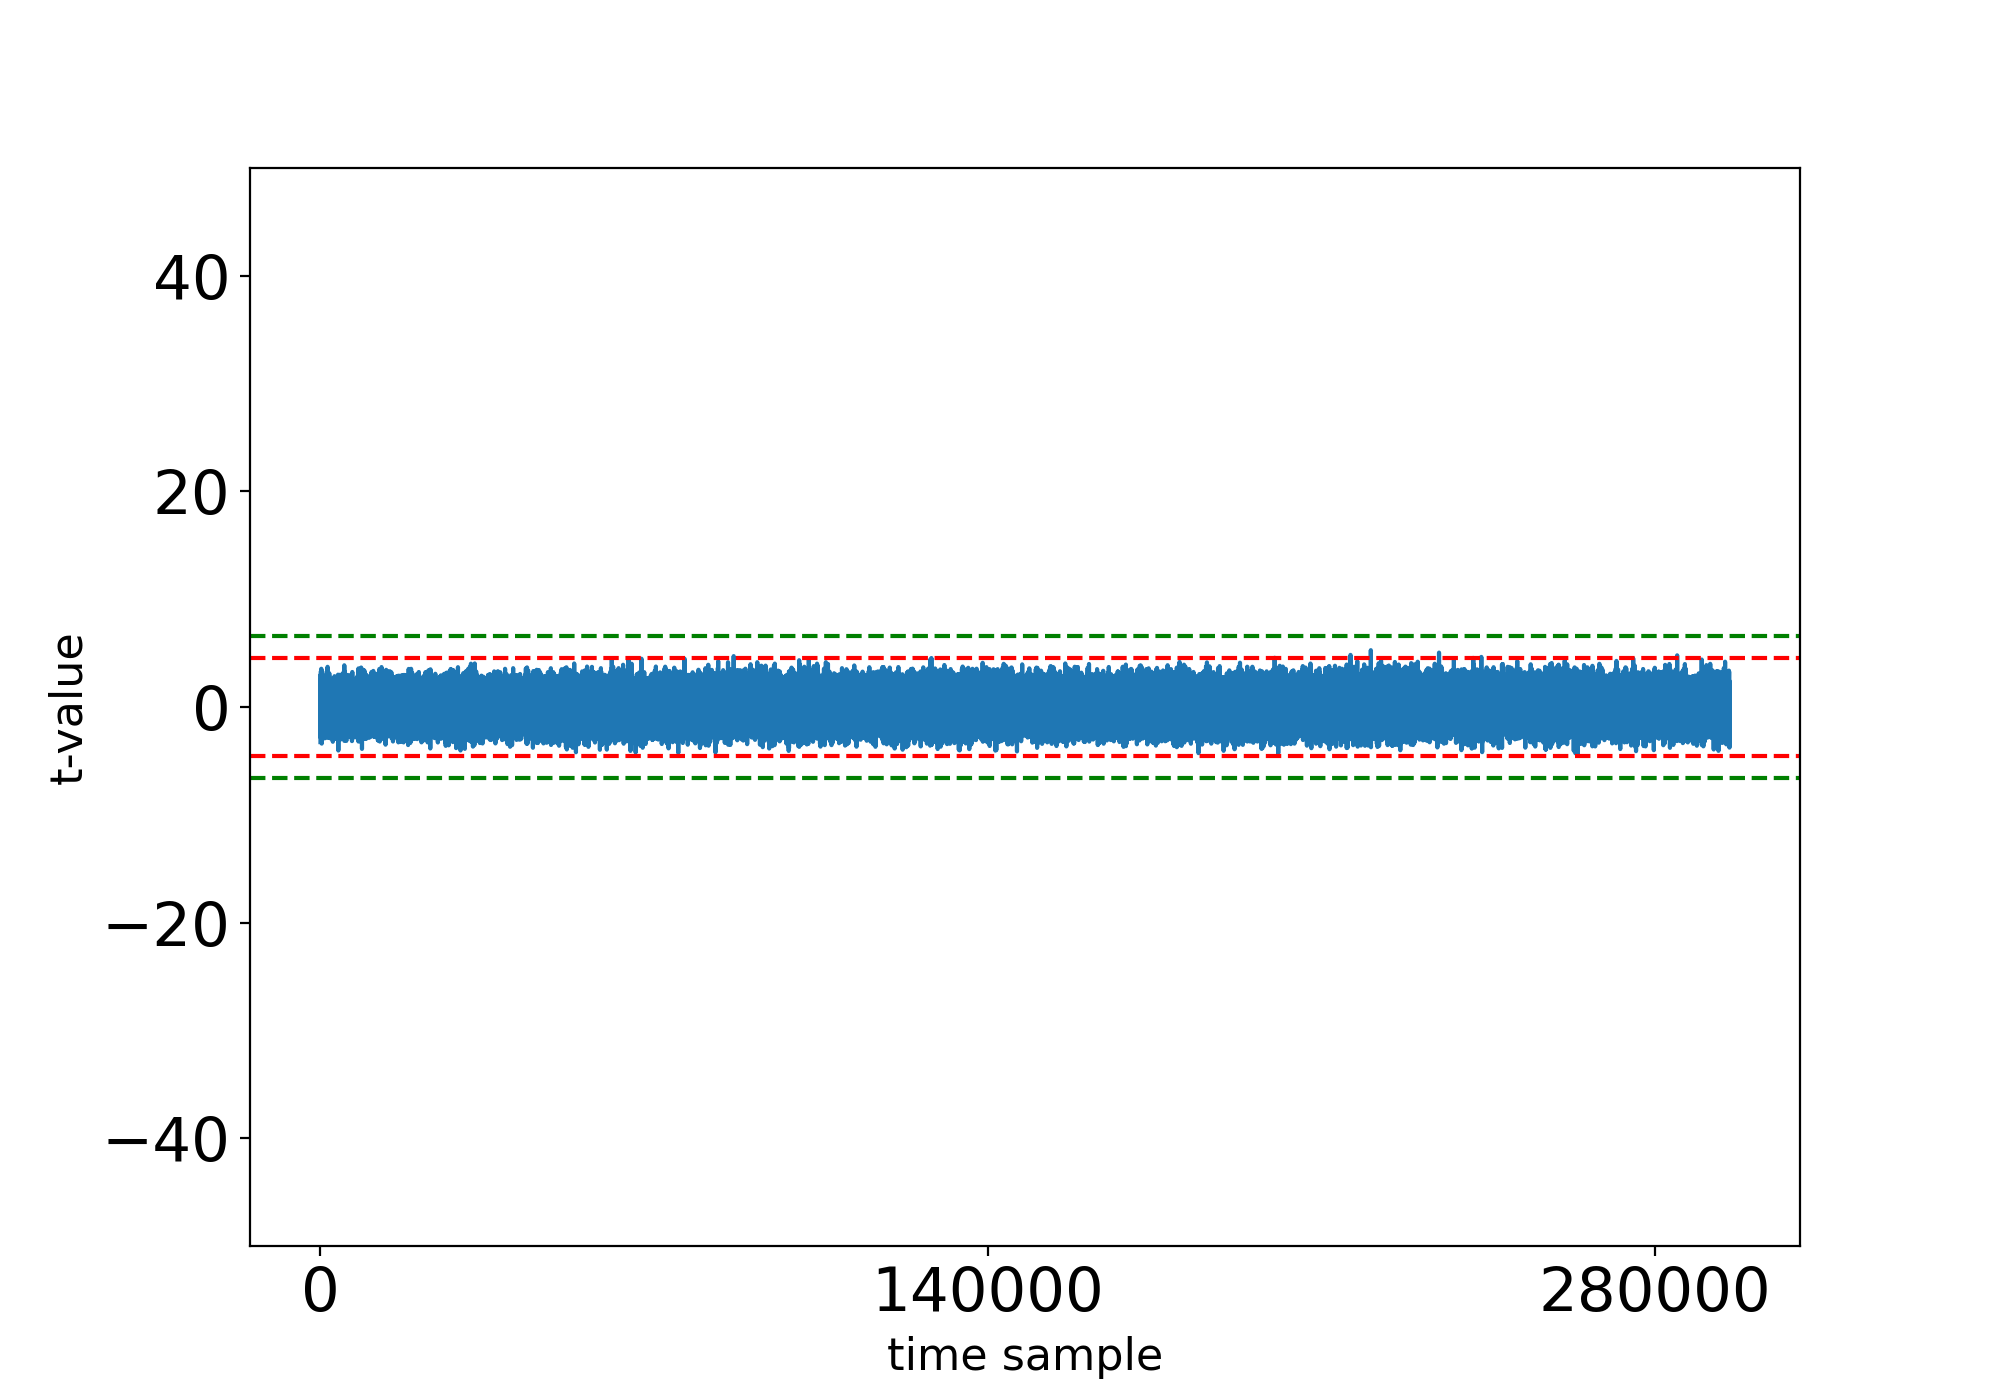
\includegraphics[width=\textwidth]{figure/tvla/SecFprMul_3shares_100k.png}
\vspace{-20pt}
\caption{100,000 traces, 3-shared SecFprMul}
\end{figure}

\end{columns}


\end{frame}



\begin{frame}{TVLA}

The TVLA results of floating-point number addition (FprAdd, SecFprAdd).

\vskip -15pt
\begin{columns}[T]
\column{.34\textwidth}
\begin{figure}
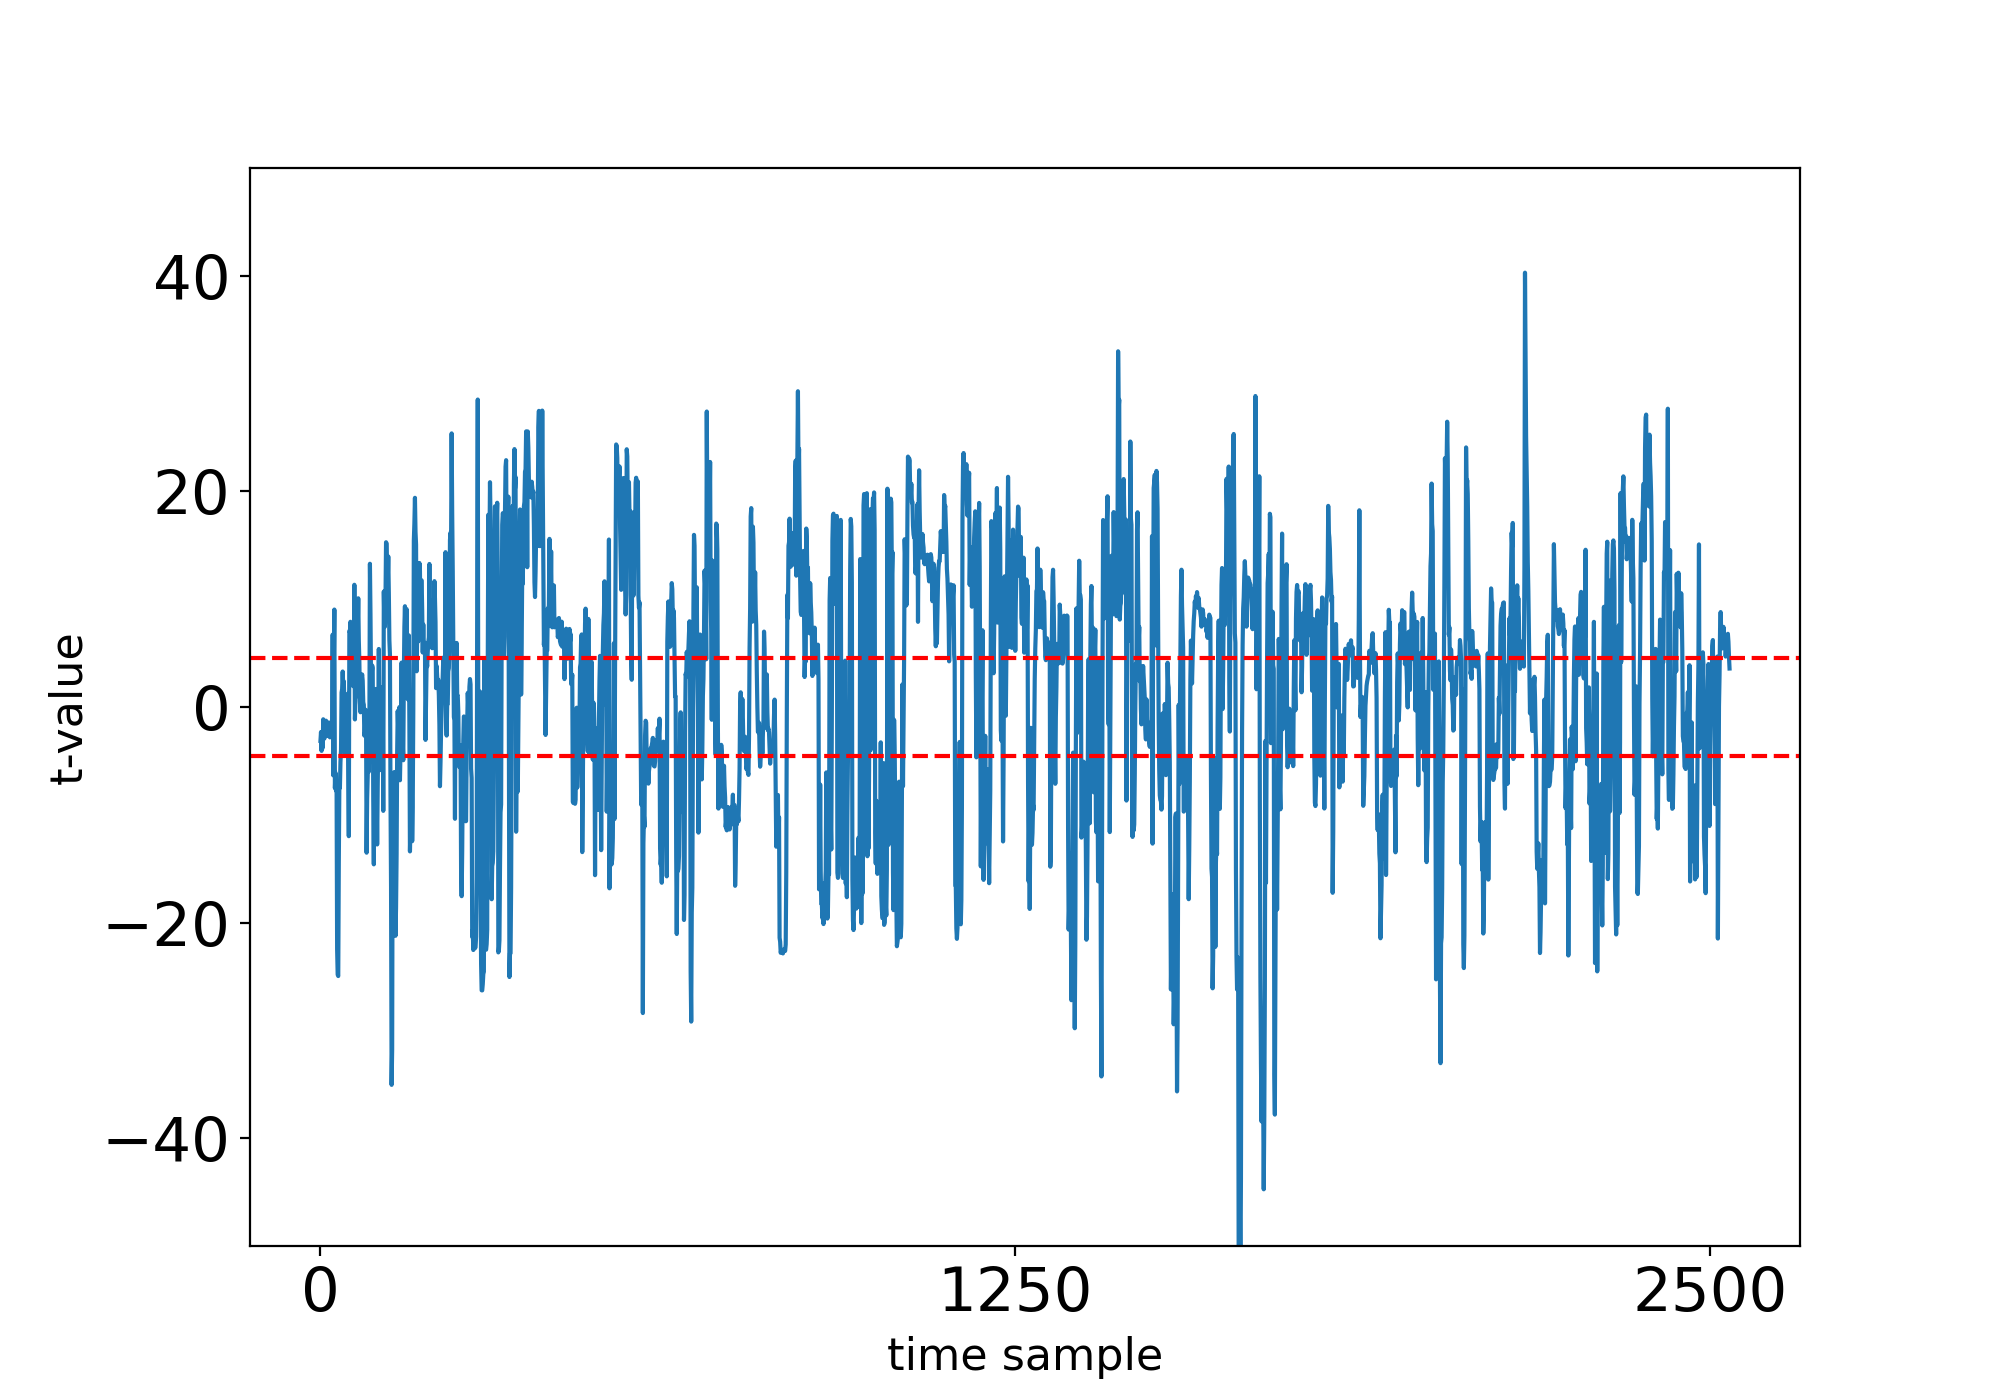
\includegraphics[width=\textwidth]{figure/tvla/fpradd_1k.png}
\vspace{-20pt}
\caption{1,000 traces, unmasked FprAdd}
\end{figure}

\column{.34\textwidth}
\begin{figure}
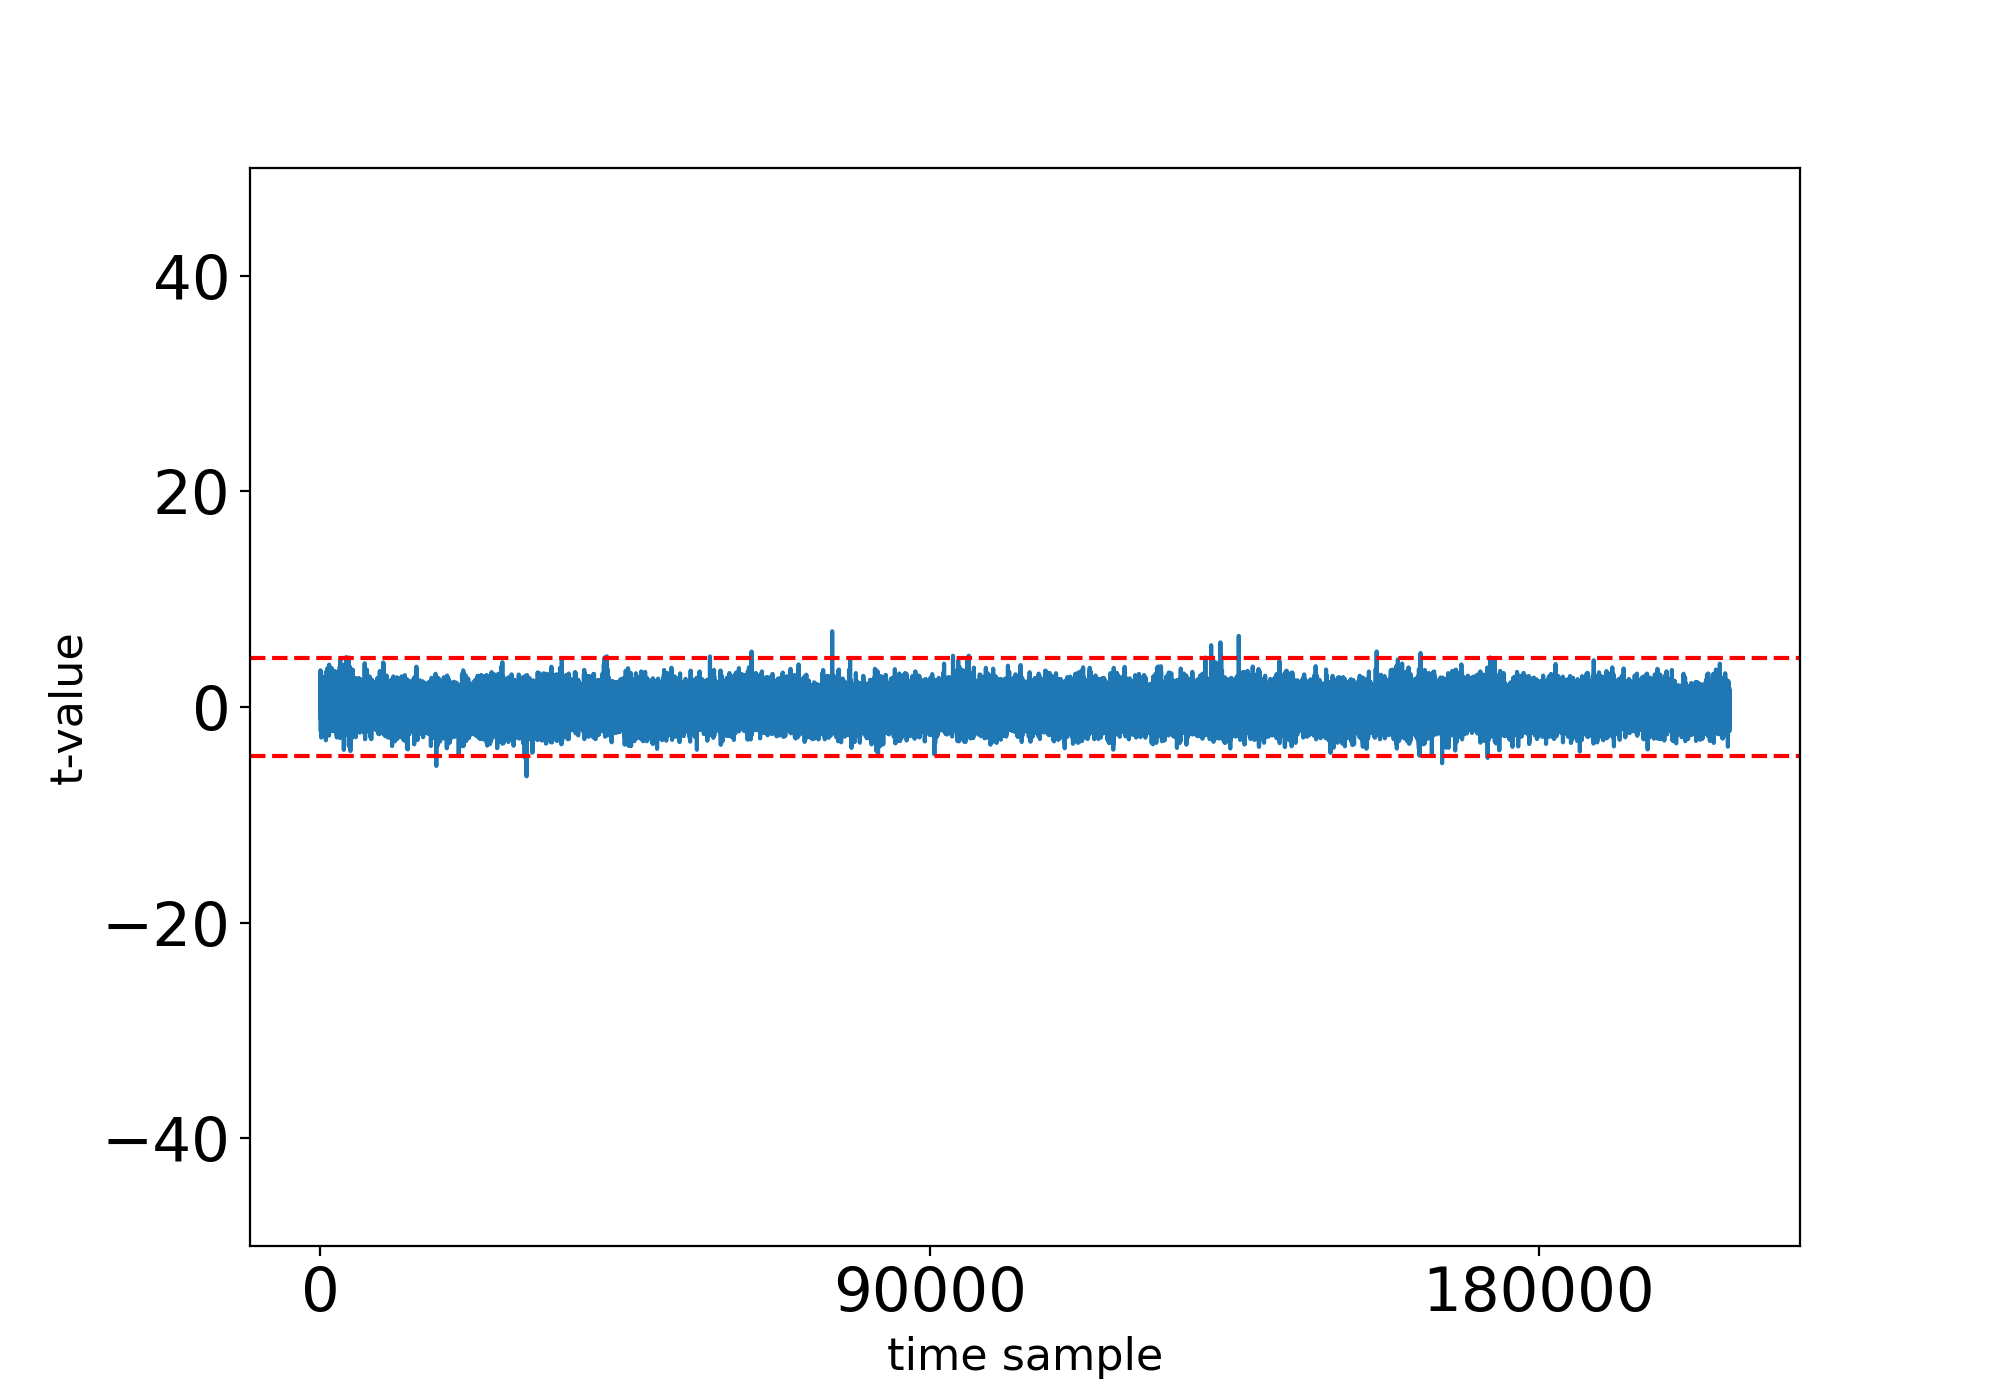
\includegraphics[width=\textwidth]{figure/tvla/1012_SecFprAdd_2shares_10k.png}
\vspace{-20pt}
\caption{10,000 traces, 2-shared SecFprAdd}
\end{figure}

\column{.34\textwidth}
\begin{figure}
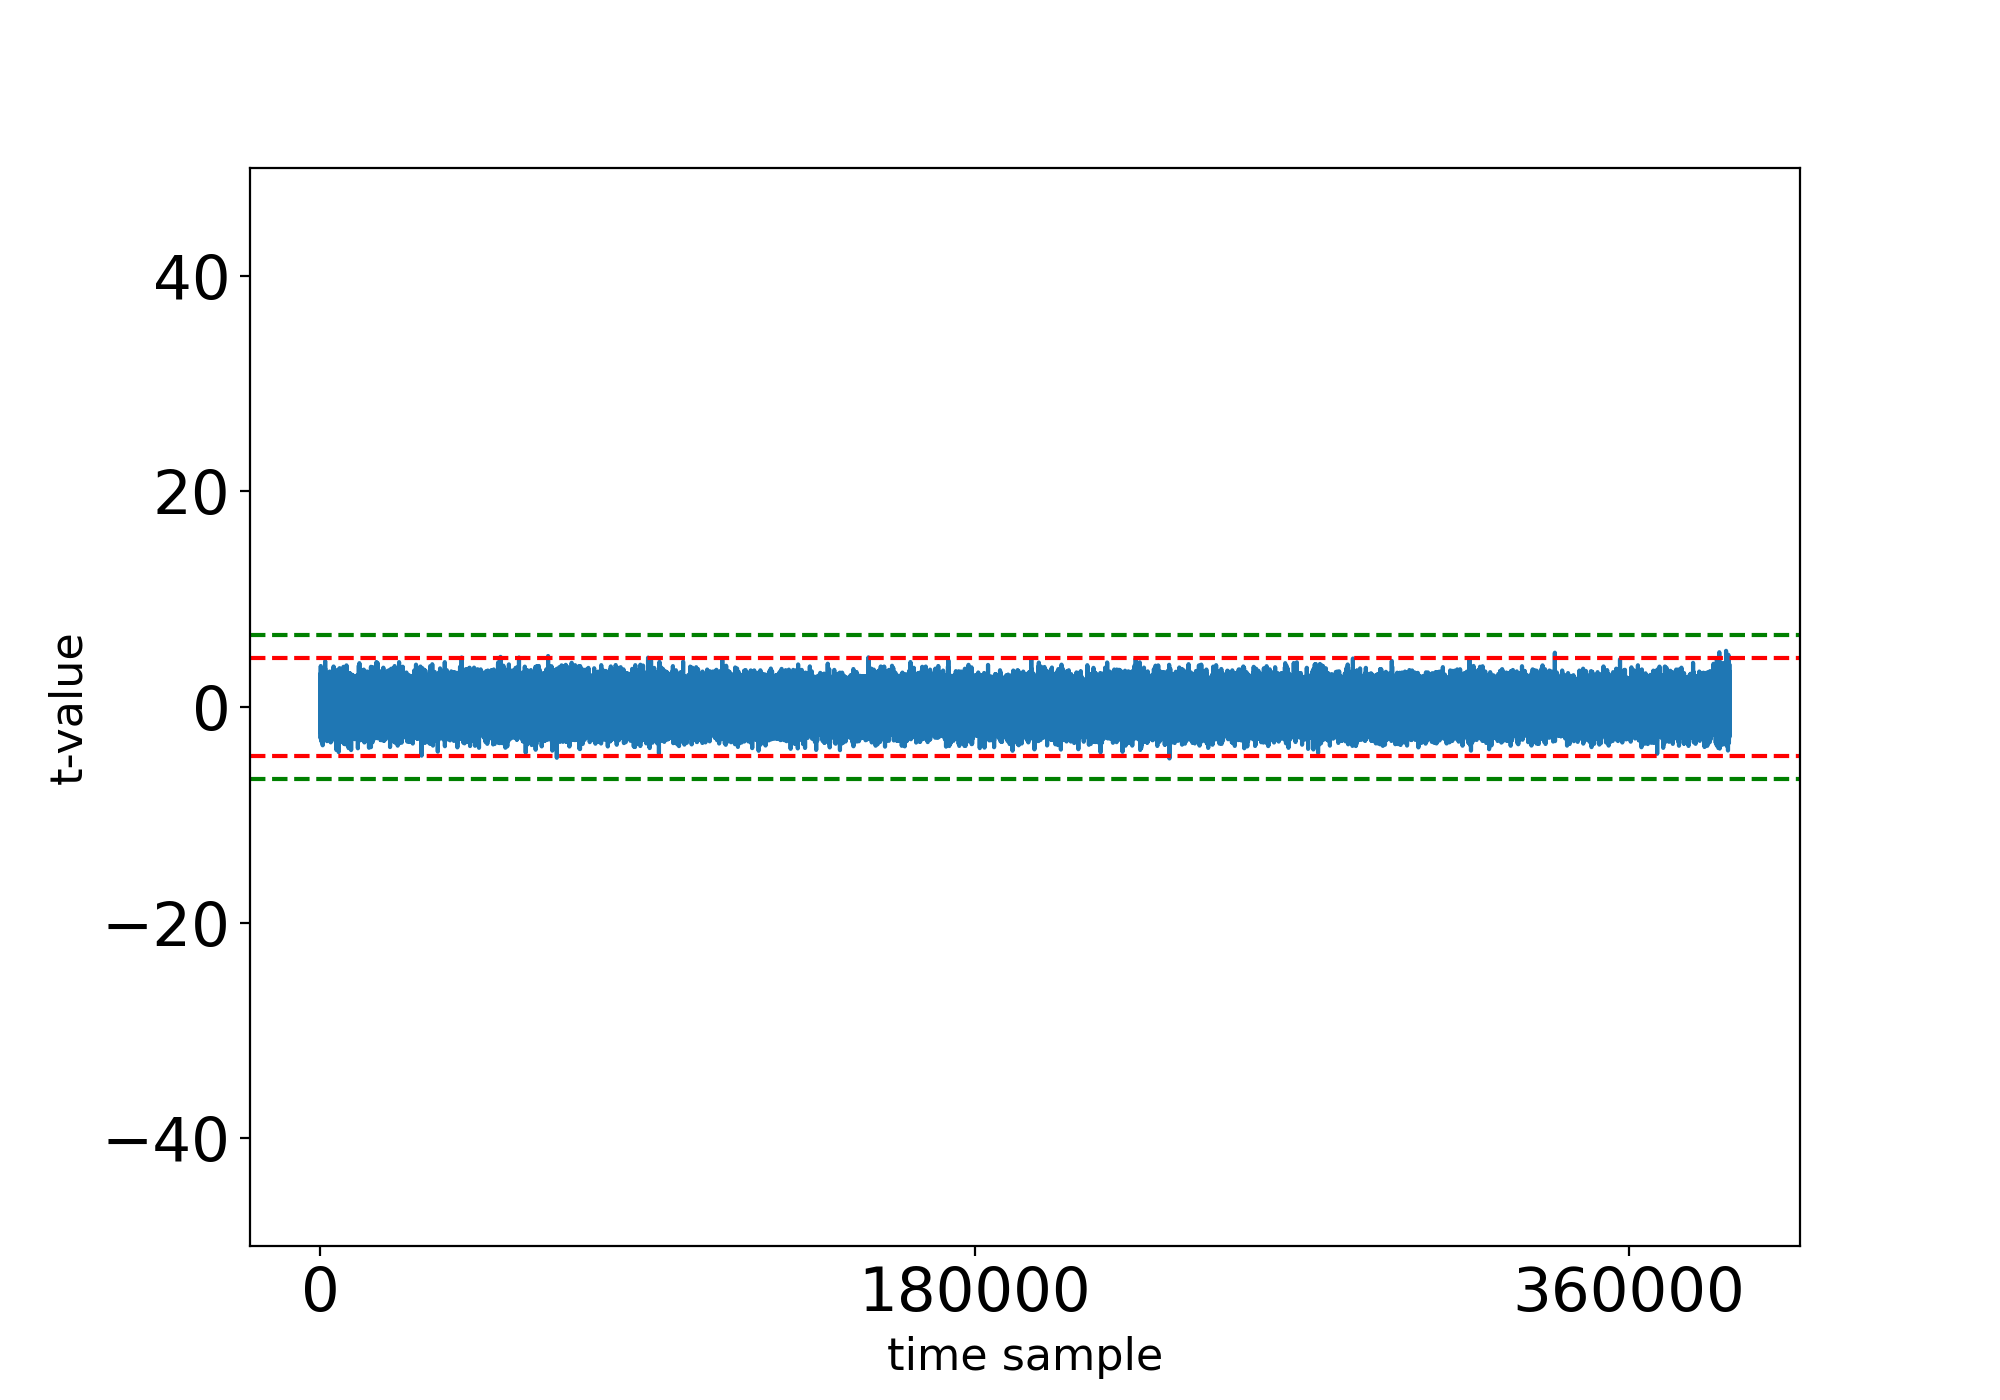
\includegraphics[width=\textwidth]{figure/tvla/SecFprAdd_3shares_100k.png}
\vspace{-20pt}
\caption{100,000 traces, 3-shared SecFprAdd}
\end{figure}

\end{columns}


\end{frame}


%
%\begin{frame}{TVLA}
%
%The 3-shared version show no obvious leakage in even 100,000 traces. We adapt the thresholds (green) \cite{ding2018towards} to $\pm 6.603$ for {\sf SecFprMul} and $\pm 6.646$ for {\sf SecFprAdd}.
%
%\vskip -15pt
%\begin{columns}[T]
%\column{.5\textwidth}
%\begin{figure}
%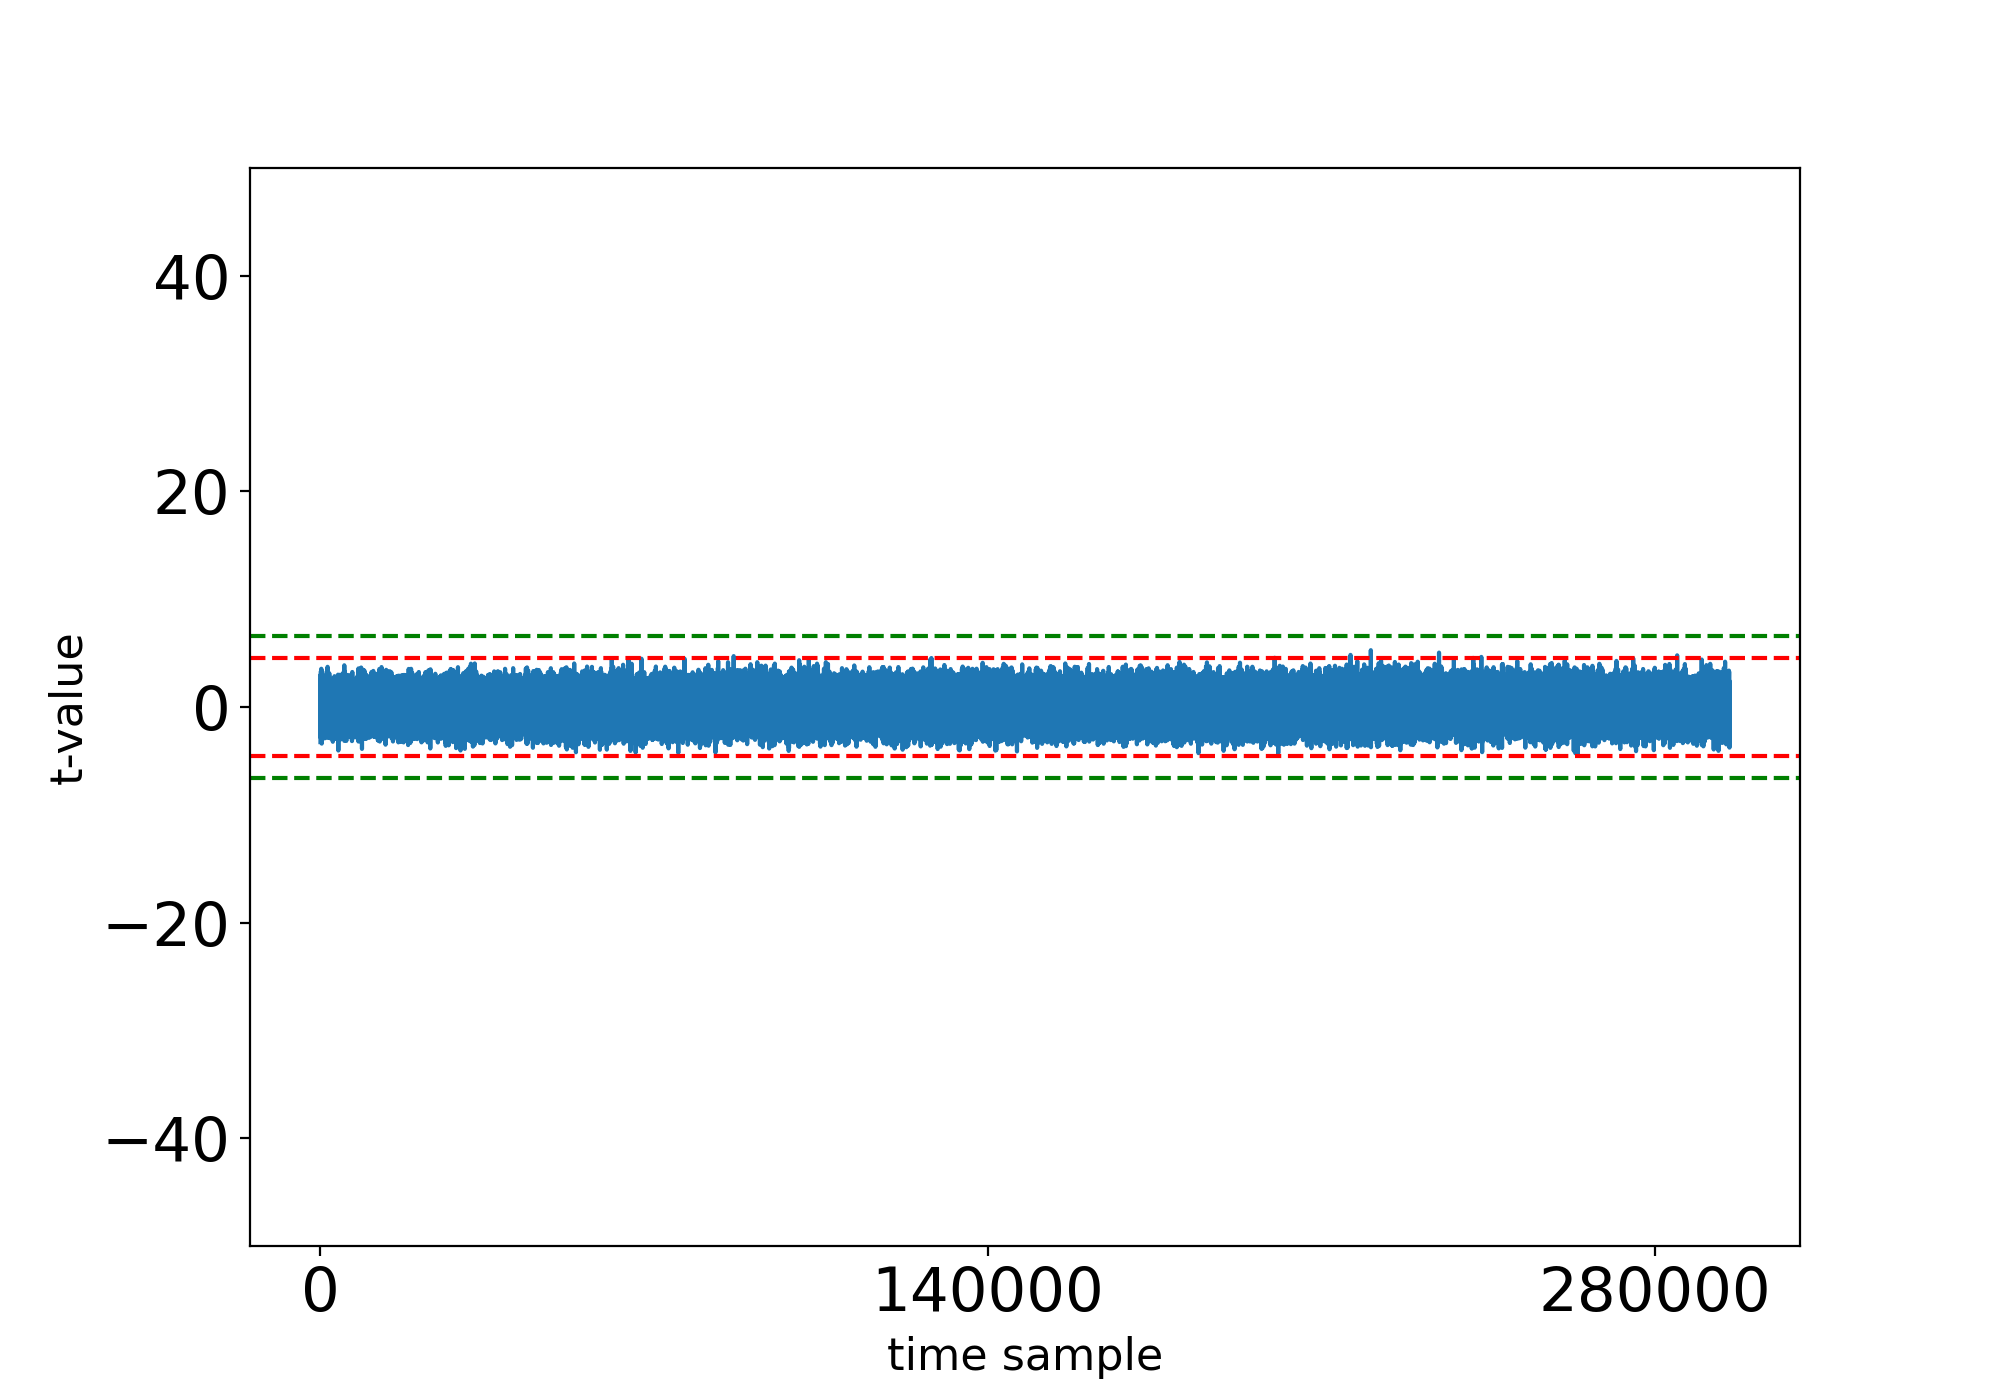
\includegraphics[width=\textwidth]{figure/tvla/SecFprMul_3shares_100k.png}
%\vspace{-20pt}
%\caption{100,000 traces, 3-shared SecFprMul}
%\end{figure}



%\end{frame}

\subsection{Performance}
\begin{frame}{Performance Evaluation on ARM Cortex-M4}

\begin{table}[ht]
\centering
\begin{tabular}{c r r@{\hspace{2pt}}l r@{\hspace{2pt}}l} 
	
	\toprule

	\multirow{2}{*}{\textbf{Gadget}} & \multicolumn{5}{c}{\textbf{Cycle}} \\
	\cline{2-6}
	& \textbf{Unmasked} & \multicolumn{2}{c}{\textbf{2 Shares}} & \multicolumn{2}{c}{\textbf{3 Shares}} \\
	
	\midrule

	{\sf FprMul/SecFprMul}
	& 308 & 7134 & ($23 \times$)  & 36388 & ($118 \times$)  \\

	\midrule

	{\sf FprAdd/SecFprAdd}
	& 487 & 17154 & ($35 \times$)  & 48291 & ($99 \times$) \\

	\bottomrule

\medskip
\end{tabular}
\caption{Performance evaluation of SecFprMul and SecFprAdd}
\label{table:performance:overall}
\end{table}


\end{frame}


\begin{frame}{Performance Evaluation on Intel-Core i9-12900KF}
\medskip

We also test the time for signing one message on a general-purpose CPU.
\medskip

\begin{table}
\centering
\begin{tabular}{c r r@{\hspace{2pt}}l r@{\hspace{2pt}}l} 
	
	\toprule
	
	\textbf{Security Level} & \textbf{Unmasked} & \multicolumn{2}{c}{\textbf{2 Shares}} & \multicolumn{2}{c}{\textbf{3 Shares}} \\
	
	\midrule
	
	{\sf Falcon-512} & 246.56 & 1905.55 & ($7.7 \times$) & 6137.25 & $(24.9 \times)$  \\
	{\sf Falcon-1024} & 501.62 & 3819.76 & ($7.6 \times$) & 12287.29 & $(24.5 \times)$ \\
	
	\bottomrule

\end{tabular}
\caption{Time (in microseconds) for signing a message on Intel-Core i9-12900KF CPU.}
\label{table:performance:sign}
\end{table}


\end{frame}




\section{Conclusion}

\begin{frame}{Conclusion}

In this paper,
\pause
\begin{itemize}
	\item We present the first masking algorithm for floating-point number multiplication and addition to protect the pre-image vector computation.
	\pause
	\item We design novel gadgets {\sf SecNonzero}, {\sf SecFprUrsh}, and {\sf SecFprNorm64} to mask the algorithms.
	\pause
	\item All our masked algorithms are proven $t$-NI or $t$-SNI secure – they are $t$-probing secure.
	\pause
	\item The TVLA result shows no leakage in the 2-shared version in 10,000 traces, and no leakage in the 3-shared version in 100,000 traces.
	\pause
	\item Our countermeasure when compared to the unmasked reference implementation is much slower. Improved {\sf SecAdd} and {\sf A2B} can reduce the cost.
\end{itemize}


\end{frame}


\section*{Reference}

\begin{frame}[allowframebreaks]{Reference}

% \nocite{*}

\printbibliography[title=Reference]

\end{frame}

%\section{Appendix}
\appendix
\backupbegin

% \section{Appendix - Algorithms of Floating-Point Number Arithmetic}
% \label{sec:appendix-fpu}
% \begin{frame}{Floating-Point Number Packing and Rounding}

\centerline{
\blockalgstart{.6\textwidth}{{\large FPR}}
\begin{algorithm}[H]
  \label{alg:FPR}
  \algsetup{linenosize=\small}
  \begin{algorithmic}[1]
    \REQUIRE Sign bit $s$, exponent $e$, and 55-bit mantissa $z$
    \ENSURE FPN $x$ packed by $s, e, z$
    \STATE $e \gets e + 1076$
    \STATE $b \gets \llbracket e < 0 \rrbracket$
    \STATE $z \gets z \wedge (b-1)$
    \STATE $b \gets \llbracket z \neq 0 \rrbracket $
    \STATE $e \gets e \wedge (-b)$
    \STATE $x \gets ((s \ll 63) \vee (z \gg 2)) + e \ll 52$
    \STATE $f \gets {\tt0XC8} \gg z^{[3:1]} $
    \STATE $x \gets x + f^{(1)}$ \COMMENT{increment if $z^{[3:1]}$ is 011,110 or 111} \\ 
    \RETURN \hskip -4pt $x$
  \end{algorithmic}
\end{algorithm}
\blockalgend
}

\end{frame}


\begin{frame}{Floating-Point Number Multiplication}

\centerline{
\blockalgstart{.9\textwidth}{{\large FprMul}}
\begin{algorithm}[H]
  \label{alg:fpr_mul}
  \algsetup{linenosize=\small}
  \begin{multicols}{2}
  \begin{algorithmic}[1]
    \REQUIRE FPN $x = (sx, ex, mx)$
    \REQUIRE FPN $y = (sy, ey, my)$
    \ENSURE FPN product of $x$ and $y$
    \STATE $s \gets sx \oplus sy$ \label{alg:FprMul:signbit}
    \STATE $e \gets ex + ey - 2100$ \label{alg:FprMul:exponent}
    \STATE $z \gets mx \times my$ \label{alg:FprMul:mantissa}
    \STATE $b \gets \llbracket z^{[50:1]} \neq 0 \rrbracket$
    \STATE $z \gets z^{[106:51]} \vee b$
    \STATE $z' \gets (z \gg 1) \vee z^{(1)}$
    \STATE $w \gets z^{(106)}$
    \STATE $z \gets z \oplus (z \oplus z') \wedge (-w)$
    \STATE $e \gets e + w$
    \STATE $bx \gets \llbracket ex \neq 0 \rrbracket$, $by \gets \llbracket ey \neq 0 \rrbracket$
    \STATE $b \gets bx \wedge by$
    \STATE $z \gets z \wedge (-b)$ \\
    \RETURN \hskip -4pt ${\sf FPR}(s, e, z)$
  \end{algorithmic}
  \end{multicols}
\end{algorithm}
\vspace{-10pt}
\blockalgend
}

\end{frame}


\begin{frame}{Floating-Point Number Addition}

\centerline{
\blockalgstart{.9\textwidth}{{\large FprAdd}}
\begin{algorithm}[H]
  \label{alg:fpr_add}
  \algsetup{linenosize=\small}
  \begin{multicols}{2}
  \small
  \begin{algorithmic}[1]
    \REQUIRE FPNs $x$ and $y$
    \ENSURE FPN sum of $x$ and $y$
    \STATE $d \gets x^{[63:1]} - y^{[63:1]}$
    \STATE $cs \gets d^{(64)} \vee ((1 - (-d)^{(64)}) \wedge x^{(64)}) $
    \STATE $m \gets (x \oplus y) \wedge (-cs)$
    \STATE $x \gets x \oplus m, y \gets y \oplus m$
    \STATE Extract $(sx, ex, mx)$ and $(sy, ey, my)$ from $x, y$, respectively.
    \STATE $mx \gets mx \ll 3, my \gets my \ll 3$
    \STATE $ex \gets ex - 1078, ey \gets ey - 1078$
    \STATE $c \gets ex - ey$
    \STATE $b \gets \llbracket c < 60 \rrbracket$ \label{alg:FprAdd:large_exp_start}
    \STATE $my \gets my \wedge (-b) $ \label{alg:FprAdd:large_exp_end}
    \STATE $my \gets (my \gg c) \vee \llbracket my^{[c:1]} \neq 0 \rrbracket$ \label{alg:FprAdd:unsigned-right-shift}
    \STATE $s \gets sx \oplus sy$
    \STATE $z \gets mx + (-1)^s my $
    \STATE Normalize $z, ex$ to make the 64th bit of $z$ set \label{alg:FprAdd:normalize}
    \STATE $z \gets (z \gg  9) \vee \llbracket z^{[9:1]} \neq 0 \rrbracket$
    \STATE $ex \gets ex + 9$ \\
    \RETURN \hskip -4pt ${\sf FPR}(sx, ex, z)$
  \end{algorithmic}
  \end{multicols}
\end{algorithm}
\vspace{-10pt}
\blockalgend
}

\end{frame}

\section{Appendix – Details of Our Design}
\label{sec:appendix}
\hypertarget{sec:appendix}{}

\subsection{New Gadgets}
\begin{frame}{SecNonzero}

We need a gadget that, given shares $(x_i)_{i=1}^n$, can derive one-bit shares $(b_i)_{i=1}^n$  such that
\[
\left \llbracket \bigoplus_{i=1}^n x_i \neq 0 \right\rrbracket = \bigoplus_{i=1}^n b_i \quad \text{or} \quad \textcolor<2->{trans}{\left \llbracket \sum_{i=1}^n x_i \neq 0 \right\rrbracket = \bigoplus_{i=1}^n b_i}
\]
\pause
For Boolean shares, our method is by considering OR-ing all the bits.
\[
 x = 0  \Longleftrightarrow x^{(k)} \vee x^{(k-1)} \vee \cdots \vee x^{(1)} = 0
\]
\pause
Now we turn to a gadget for secure OR operations.
    
\end{frame}


\begin{frame}{SecOr: OR of Boolean Shares}

\centerline{
\blockalgstart{.6\textwidth}{{\large SecOr}}
\begin{algorithm}[H]
  \label{alg:SecOr}
  \algsetup{linenosize=\small}
  \begin{algorithmic}[1]
    \REQUIRE Boolean shares $(x_i)_{1\leq i \leq n}$ for value $x$
    \REQUIRE Boolean shares ${(y_i)_{1 \leq i \leq n}}$ for value $y$
    \ENSURE Boolean shares ${(z_i)_{1 \leq i \leq n}}$ for value $z = x \vee y$
    \STATE ${(t_i)_{1\leq i \leq n} \gets  (\neg x_1, x_2, \cdots, x_n)}$
    \STATE ${(s_i)_{1\leq i \leq n} \gets  (\neg y_1, y_2, \cdots, y_n)}$
    \STATE $(z_i) \gets {\sf SecAnd} ( (s_i), (t_i) ) $
    \STATE $z_1 \gets \neg z_1$
    \STATE \Return $( z_i )$  \end{algorithmic}
\end{algorithm}
\vspace{-5pt}
\blockalgend
}
\medskip
It applies De Morgan's law and calls the AND algorithm ${\sf SecAnd}$ of shares as a subroutine.
\[
x \vee y = \neg \left[ (\neg x) \wedge (\neg y) \right]
\]

\end{frame}


\begin{frame}{SecNonzero}

For arithmetic shares, instead of applying an $n$-shared {A2B}, we consider that
\[
\sum_{i=1}^{n} x_i = 0  \Longleftrightarrow  \sum_{i=1}^{\frac{n}{2}} x_i = \sum_{i=\frac{n}{2}+1}^{n} (-x_i) \Longleftrightarrow \sum_{i=1}^{\frac{n}{2}} x_i \oplus \sum_{i=\frac{n}{2}+1}^{n} (-x_i) = 0
\]
\pause
So we apply two $n/2$-shared {\sf A2B}s to the first $n/2$ shares and negative of the second $n/2$ shares and use the same idea.
\pause
\medskip

In this way, we replace one $n$-shared {A2B} with two $n/2$-shared {\sf A2B}s, which is usually more efficient.
    
\end{frame}


\begin{frame}{SecNonzero}

\centerline{
\blockalgstart{.7\textwidth}{{\large SecNonzero}}
\begin{algorithm}[H]
  \label{alg:SecNonzero}
  \algsetup{linenosize=\small}
  \small
  \begin{algorithmic}[1]
    \REQUIRE Shares ${(x_i)_{1\leq i \leq n}}$ for value $x$, ${\sf bitsize}$
    \ENSURE One-bit Boolean shares ${ (b_i)_{1\leq i \leq n}}$ where $\bigoplus_i b_i = 0 \Leftrightarrow x = 0$
    \IF{input $(x_i)$ are arithmetic shares}
        \STATE $(t_i)_{1\leq i \leq \frac{n}{2}} \gets {\sf A2B}( (x_i)_{1\leq i \leq \frac{n}{2}} )$
        \STATE $(t_i)_{\frac{n}{2}+1 \leq i \leq n} \gets {\sf A2B}( (-x_i)_{\frac{n}{2}+1 \leq i \leq n} )$
    \ELSE
        \STATE $(t_i)_{1\leq i \leq n} \gets (x_i)_{1\leq i \leq n}$
    \ENDIF
    \STATE ${\sf len} \gets {\sf bitsize} / 2$
    \WHILE{${\sf len} \geq 1$}
        \STATE $(l_i) \gets {\sf Refresh}( (t_i^{[2 {\sf len}: {\sf len}]}), {\sf len})$
        \STATE $(r_i) \gets (t_i^{[{\sf len}:1]})$
        \STATE $(t_i) \gets {\sf SecOr}((l_i), (r_i))$
        \STATE ${\sf len} \gets {\sf len} \gg 1 $
    \ENDWHILE
    \STATE \Return $(t_i^{(1)})$
\end{algorithmic}
\end{algorithm}
\vspace{-5pt}
\blockalgend
}

\end{frame}


\iffalse
%
%
%
\begin{frame}{SecNonzero in Masking FPR}

\centerline{
\blockalgstart{.6\textwidth}{{\large FPR}}
\begin{algorithm}[H]
  \algsetup{linenosize=\small}
  \begin{algorithmic}[1]
    \REQUIRE Sign bit $s$, exponent $e$, and 55-bit mantissa $z$
    \ENSURE FPN $x$ packed by $s, e, z$
    \STATE $e \gets e + 1076$
    \STATE $b \gets \llbracket e < 0 \rrbracket$
    \STATE $z \gets z \wedge (b-1)$
    \STATE \textcolor{red}{$b \gets \llbracket z \neq 0 \rrbracket $}
    \STATE $e \gets e \wedge (-b)$
    \STATE $x \gets ((s \ll 63) \vee (z \gg 2)) + e \ll 52$
    \STATE $f \gets {\tt0XC8} \gg z^{[3:1]} $
    \STATE $x \gets x + f^{(1)}$ \COMMENT{increment if $z^{[3:1]}$ is 011,110 or 111} \\ 
    \RETURN \hskip -4pt $x$
  \end{algorithmic}
\end{algorithm}
\blockalgend
}

\end{frame}


\begin{frame}{SecNonzero in Masking FprMul}

\centerline{
\blockalgstart{.9\textwidth}{{\large FprMul}}
\begin{algorithm}[H]
  \algsetup{linenosize=\small}
  \begin{multicols}{2}
  \begin{algorithmic}[1]
    \REQUIRE FPN $x = (sx, ex, mx)$
    \REQUIRE FPN $y = (sy, ey, my)$
    \ENSURE FPN product of $x$ and $y$
    \STATE $s \gets sx \oplus sy$ 
    \STATE $e \gets ex + ey - 2100$ 
    \STATE $z \gets mx \times my$
    \STATE \textcolor{red}{$b \gets \llbracket z^{[50:1]} \neq 0 \rrbracket$}
    \STATE $z \gets z^{[106:51]} \vee b$
    \STATE $z' \gets (z \gg 1) \vee z^{(1)}$
    \STATE $w \gets z^{(106)}$
    \STATE $z \gets z \oplus (z \oplus z') \wedge (-w)$
    \STATE $e \gets e + w$
    \STATE \textcolor{red}{$bx \gets \llbracket ex \neq 0 \rrbracket$}, \textcolor{red}{$by \gets \llbracket ey \neq 0 \rrbracket$}
    \STATE $b \gets bx \wedge by$
    \STATE $z \gets z \wedge (-b)$ \\
    \RETURN \hskip -4pt ${\sf FPR}(s, e, z)$
  \end{algorithmic}
  \end{multicols}
\end{algorithm}
\vspace{-10pt}
\blockalgend
}

\end{frame}


\begin{frame}{SecNonzero in Masking FprAdd}

\centerline{
\blockalgstart{.9\textwidth}{{\large FprAdd}}
\begin{algorithm}[H]
  \algsetup{linenosize=\small}
  \begin{multicols}{2}
  \small
  \begin{algorithmic}[1]
    \REQUIRE FPNs $x$ and $y$
    \ENSURE FPN sum of $x$ and $y$
    \STATE $d \gets x^{[63:1]} - y^{[63:1]}$
    \STATE $cs \gets d^{(64)} \vee ((1 - (-d)^{(64)}) \wedge x^{(64)}) $
    \STATE $m \gets (x \oplus y) \wedge (-cs)$
    \STATE $x \gets x \oplus m, y \gets y \oplus m$
    \STATE Extract $(sx, ex, mx)$ and $(sy, ey, my)$ from $x, y$, respectively.
    \STATE $mx \gets mx \ll 3, my \gets my \ll 3$
    \STATE $ex \gets ex - 1078, ey \gets ey - 1078$
    \STATE $c \gets ex - ey$
    \STATE $b \gets \llbracket c < 60 \rrbracket$ 
    \STATE $my \gets my \wedge (-b) $ 
    \STATE \textcolor{red}{$my \gets (my \gg c) \vee \llbracket my^{[c:1]} \neq 0 \rrbracket$}
    \STATE $s \gets sx \oplus sy$
    \STATE $z \gets mx + (-1)^s my $
    \STATE Normalize $z, ex$ to make the 64th bit of $z$ set
    \STATE \textcolor{red}{$z \gets (z \gg  9) \vee \llbracket z^{[9:1]} \neq 0 \rrbracket$}
    \STATE $ex \gets ex + 9$ \\
    \RETURN \hskip -4pt ${\sf FPR}(sx, ex, z)$
  \end{algorithmic}
  \end{multicols}
\end{algorithm}
\vspace{-10pt}
\blockalgend
}

\end{frame}
%
%
%
\fi


\begin{frame}{SecFprUrsh}

%
%
%
\iffalse
Given 64-bit shares $(x_i)$ and 6-bit shares $(c_i)$, we need to derive shares $(z_i)$ such that
\[
\bigoplus_{i=1}^n z_i = \left( \left( \bigoplus_{i=1}^n x_i \right) \gg \left( \sum_{i=1}^n c_i \bmod 2^{6} \right) \right) \vee \left \llbracket \bigoplus_{i=1}^n x_i^{[c:1]} \neq 0 \right \rrbracket
\]
%
%
%
\fi

Given 64-bit shares $(x_i)$ and 6-bit shares $(c_i)$, we need to derive shares $(z_i)$ such that
\[
\bigoplus_{i=1}^n z_i = \left( \bigoplus_{i=1}^n x_i \right) \gg \left( \sum_{i=1}^n c_i \bmod 64 \right)
\]

\pause
\medskip

We observe that
\pause
\begin{itemize}

\item Right-shifting and right-rotating by a value $c$ only differ by the most $c$ significant bits.
\pause
\item Right-rotating $x$ by a value $c$ is equal to right-rotating $x$ by $c \bmod 64$.
\end{itemize}

\end{frame}


\begin{frame}{SecFprUrsh}

Hence, our idea is to right-rotate all $x_i's$ by $c_1, c_2, \cdots, c_n$ sequentially.
\pause
\medskip

Some high bits are redundant, so we use an index $m = (1 \ll 63)$ to indicate the first meaningful bit of the result.
\pause
Consider
\[
m \gg c = (\underbrace{0 \cdots 0}_{c \text{ bits}} 1 0 \cdots 0)_2
\]
\pause
\[
m' := m \gg c \oplus (m \gg c) \gg 1 \oplus \cdots \oplus (m \gg c) \gg 63 = (\underbrace{0 \cdots 0}_{c \text{ bits}} 1 1 \cdots 1)_2
\]
\pause
By an AND operation with $m'$, we can clear useless bits.

\end{frame}


%
%
%
\iffalse

\begin{frame}{SecFprUrsh}

\centerline{
\blockalgstart{.9\textwidth}{{\large SecFprUrsh}}
\begin{algorithm}[H]
  \label{alg:SecFprUrsh}
  \algsetup{linenosize=\small}
  \small
  \begin{multicols}{2}
  \begin{algorithmic}[1]
    \REQUIRE 64-bit Boolean shares ${(x_i)_{1\leq i \leq n}}$
    \REQUIRE 6-bit arithmetic shares ${(c_i)_{1\leq i \leq n}}$
    \ENSURE Boolean shares ${(z_i)_{1\leq i \leq n}}$ for value $z = x \gg c$ with the sticky bit preserved
    \STATE ${(m_i)_{1\leq i \leq n}} \gets ((1 \ll 63), 0, \cdots, 0)$
    \FOR{$j = 1$ to $n$}
        \STATE Right-rotate $(x_i)$ by $c_j$
        \STATE $(x_i) \gets {\sf RefreshMasks}((x_i))$
        \STATE Right-rotate $(m_i)$ by $c_j$
        \STATE $(m_i) \gets {\sf RefreshMasks}((m_i))$
    \ENDFOR
    \STATE ${\sf len} \gets 1$
    \WHILE{${\sf len} \leq 32$}
        \STATE $(m_i) \gets (m_i \oplus (m_i \gg {\sf len}))$
        \STATE ${\sf len} \gets {\sf len} \ll 1 $
    \ENDWHILE
    \STATE $(y_i) \gets {\sf SecAnd}( (x_i), (m_i) )$
    \STATE $(z_i) \gets (y_i \oplus x_i \oplus y_i^{(1)})$
    \STATE $(b_i) \gets {\sf SecNonzero}( (z_i) )$
    \STATE $(z_i) \gets  (y_i^{[64:2]} \vee b_i) $
    \STATE \Return $(z_i)$
\end{algorithmic}
\end{multicols}
\end{algorithm}
\vspace{-10pt}
\blockalgend
}

\end{frame}


\begin{frame}{SecFprUrsh in Masking FprAdd}

\centerline{
\blockalgstart{.8\textwidth}{{\large FprAdd}}
\begin{algorithm}[H]
  \algsetup{linenosize=\small}
  \begin{multicols}{2}
  \small
  \begin{algorithmic}[1]
    \REQUIRE FPNs $x$ and $y$
    \ENSURE FPN sum of $x$ and $y$
    \STATE $d \gets x^{[63:1]} - y^{[63:1]}$
    \STATE $cs \gets d^{(64)} \vee ((1 - (-d)^{(64)}) \wedge x^{(64)}) $
    \STATE $m \gets (x \oplus y) \wedge (-cs)$
    \STATE $x \gets x \oplus m, y \gets y \oplus m$
    \STATE Extract $(sx, ex, mx)$ and $(sy, ey, my)$ from $x, y$, respectively.
    \STATE $mx \gets mx \ll 3, my \gets my \ll 3$
    \STATE $ex \gets ex - 1078, ey \gets ey - 1078$
    \STATE $c \gets ex - ey$
    \STATE $b \gets \llbracket c < 60 \rrbracket$ 
    \STATE $my \gets my \wedge (-b) $ 
    \STATE \textcolor{red}{$my \gets (my \gg c) \vee \llbracket my^{[c:1]} \neq 0 \rrbracket$}
    \STATE $s \gets sx \oplus sy$
    \STATE $z \gets mx + (-1)^s my $
    \STATE Normalize $z, ex$ to make the 64th bit of $z$ set
    \STATE $z \gets (z \gg  9) \vee \llbracket z^{[9:1]} \neq 0 \rrbracket$
    \STATE $ex \gets ex + 9$ \\
    \RETURN \hskip -4pt ${\sf FPR}(sx, ex, z)$
  \end{algorithmic}
  \end{multicols}
\end{algorithm}
\vspace{-10pt}
\blockalgend
}

\end{frame}

\fi

\begin{frame}{SecFprNorm64}

Given 64-bit shares $(x_i)$ and 16-bit shares $(e_i)$, we need to derive new $(x_i')$ and $(e_i')$ such that
\[
\text{Let } c \text{ be the smallest integer such that } \left( (\oplus_{i=1}^n x_i) \ll c \right) \in [2^{63}, 2^{64})
\]
\[
\text{then } (\oplus_{i=1}^n x_i') = \left( (\oplus_{i=1}^n x_i) \ll c \right) \text{ and } \sum_{i=1}^n e_i' = (\sum_{i=1}^n e_i) - c
\]
\pause

We can repeatedly check whether $(x^{(64)}_i)$ is $0$, then conditionally shift by $1$ bit, and then decrease $(e_i)$ by $\llbracket (x^{(64)}_i) = 0 \rrbracket$.
\pause

To improve efficiency, we consider sequentially checking $x^{[64:64-2^j]} = 0$ for $j = 5,4,\cdots,0$.
\pause

In addition, we first decrease $(e_i)$ by $63$ and later add $\llbracket (x^{[64:64-2^j]}_i) \neq 0 \rrbracket \cdot 2^j$ to it.
\end{frame}

\begin{frame}{SecFprNorm64}

\centerline{
\blockalgstart{.78\textwidth}{{\large SecFprNorm64}}
\begin{algorithm}[H]
  \label{alg:SecFprNorm64}
  \algsetup{linenosize=\small}
  \small
  % \begin{multicols}{2}
  \begin{algorithmic}[1]
    \REQUIRE 64-bit Boolean shares ${(x_i)_{1\leq i \leq n}}$
    \REQUIRE 16-bit arithmetic shares ${(e_i)_{1\leq i \leq n}}$
    \ENSURE Normalized ${(x_i)_{1\leq i \leq n}}$ in $[2^{63}, 2^{64})$ and ${(e_i)_{1\leq i \leq n}}$ with shift added
    \STATE $e_1 \gets e_1 - 63$
    \FOR{$j = 5$ to $0$}
        \STATE $(t_i) \gets (x_i \oplus (x_i \ll 2^j))$
        \STATE $(n_i) \gets (x_i \gg (64 - 2^j))$
        \STATE $(b_i) \gets {\sf SecNonzero}( (n_i) )$
        \STATE $(b'_i) \gets (-b_i)$
        \STATE $(t_i) \gets {\sf SecAnd}( (t_i), { (\neg b'_1, b'_2,\cdots, b'_n)} )$
        \STATE $(x_i) \gets (x_i \oplus t_i)$
        \STATE $(b_i) \gets {\sf B2A_{Bit}}( (b_i) )$
        \STATE $(e_i) \gets (e_i + (b_i \ll j))$
    \ENDFOR
    \STATE \Return $(x_i), (e_i)$
\end{algorithmic}
% \end{multicols}
\vskip -5pt
\end{algorithm}

\blockalgend
}

\end{frame}


\iffalse
%
%
%
\begin{frame}{SecFprNorm64 in Masking FprAdd}

\centerline{
\blockalgstart{.9\textwidth}{{\large FprAdd}}
\begin{algorithm}[H]
  \algsetup{linenosize=\small}
  \begin{multicols}{2}
  \small
  \begin{algorithmic}[1]
    \REQUIRE FPNs $x$ and $y$
    \ENSURE FPN sum of $x$ and $y$
    \STATE $d \gets x^{[63:1]} - y^{[63:1]}$
    \STATE $cs \gets d^{(64)} \vee ((1 - (-d)^{(64)}) \wedge x^{(64)}) $
    \STATE $m \gets (x \oplus y) \wedge (-cs)$
    \STATE $x \gets x \oplus m, y \gets y \oplus m$
    \STATE Extract $(sx, ex, mx)$ and $(sy, ey, my)$ from $x, y$, respectively.
    \STATE $mx \gets mx \ll 3, my \gets my \ll 3$
    \STATE $ex \gets ex - 1078, ey \gets ey - 1078$
    \STATE $c \gets ex - ey$
    \STATE $b \gets \llbracket c < 60 \rrbracket$ 
    \STATE $my \gets my \wedge (-b) $ 
    \STATE $my \gets (my \gg c) \vee \llbracket my^{[c:1]} \neq 0 \rrbracket$
    \STATE $s \gets sx \oplus sy$
    \STATE $z \gets mx + (-1)^s my $
    \STATE \textcolor{red}{Normalize $z, ex$ to make the 64th bit of $z$ set}
    \STATE $z \gets (z \gg  9) \vee \llbracket z^{[9:1]} \neq 0 \rrbracket$
    \STATE $ex \gets ex + 9$ \\
    \RETURN \hskip -4pt ${\sf FPR}(sx, ex, z)$
  \end{algorithmic}
  \end{multicols}
\end{algorithm}
\vspace{-10pt}
\blockalgend
}

\end{frame}
%
%
%
\fi

\subsection{SecFPR: Secure FPR}
\begin{frame}{SecFPR: Secure FPR}

\begin{columns}[T]
\column{.6\textwidth}
\begin{block}{{\large FPR}}
\begin{algorithm}[H]
  \algsetup{linenosize=\small}
  \begin{algorithmic}[1]
    \REQUIRE \textcolor<2>{red}{ Sign bit $s$, exponent $e$, and 55-bit mantissa $z$}
    \ENSURE FPN $x$ packed by $s, e, z$
    \STATE \textcolor<3>{red}{$e \gets e + 1076$}

    \STATE \textcolor<4>{red}{$b \gets \llbracket e < 0 \rrbracket$}

    \STATE \textcolor<4>{red}{$z \gets z \wedge (b-1)$}
   
    \STATE \textcolor<5>{red}{$b \gets \llbracket z \neq 0 \rrbracket $}

    \STATE \textcolor<6>{red}{ $e \gets e \wedge (-b)$ }

    \STATE \textcolor<6>{red}{ $x \gets ((s \ll 63) \vee (z \gg 2)) + e \ll 52$}

    \STATE \textcolor<7>{red}{$f \gets {\tt0XC8} \gg z^{[3:1]} $ }

    \STATE \textcolor<7>{red}{$x \gets x + f^{(1)}$} \\ 
    \RETURN \hskip -12pt \textcolor<8>{red}{$x$}
  \end{algorithmic}
\end{algorithm}
\end{block}

\column{.35\textwidth}


\only<1>{
\vskip 70pt
We now show how we mask the floating-point number rounding and packing algorithm {\sf FPR}.
}


\only<2>{
\vskip 50pt
Recall that {\sf FPR} is the last subroutine of {\sf FprMul} and {\sf FprAdd}.

By our masking design of {\sf FprMul} and {\sf FprAdd}, $(s_i)$ is Boolean-masked, $(e_i)$ is 16-bit arithmetic-masked, and $(z_i)$ is Boolean-masked.
}


\only<3>{
\vskip 70pt
This is by adding to any one share.
}


\only<4>{
\vskip 50pt
This is equivalent to
\centerline{
\blockalgstart{.6\textwidth}{}
\begin{algorithm}[H]
  \algsetup{linenosize=\small}
  \begin{algorithmic}[1]
    \IF{$e < 0$}
        \STATE $z \gets 0$
    \ENDIF
\end{algorithmic}
\end{algorithm}
\blockalgend
}

\medskip
and is done by an ${\sf A2B}$, taking the MSB, and the simple trick.
}


\only<5>{
\vskip 70pt
This is done by {\sf SecNonzero} and the simple trick.
}


\only<6>{
\vskip 50pt
Shift, OR, and a {\sf SecAdd}.

We add $(e_i)$ and the $55$th bit of $(z_i)$ in advance instead of adding $(e_i)$ to a 64-bit value. That is, use a 16-bit {\sf SecAdd} to save a 64-bit {\sf SecAdd} 
}


\only<7>{
\vskip 50pt
If the least 3 bits of $(z_i)$ are 011, 110, and 111, $f^{(1)} = 1$.

We OR $(z^{(1)}_i)$ and $(z^{(3)}_i)$ by {\sf SecOr}, and then AND $(z^{(2)}_i)$ by {\sf SecAnd}. The result is then added to $(x_i)$ by {\sf SecAdd}.
}


\only<8>{
\vskip 70pt
Done.

The returned value is a 64-bit Boolean-masked $(x_i)$.
}

\end{columns}

\end{frame}



\begin{frame}{SecFPR: Secure FPR}

\centerline{
\blockalgstart{\textwidth}{{\large SecFPR}}
\begin{algorithm}[H]
  \algsetup{linenosize=\small}
  \label{alg:SecFPR}
  \begin{multicols}{2}
  \begin{algorithmic}[1]
    \REQUIRE 1-bit Boolean shares ${(s_i)_{1\leq i \leq n}}$
	\REQUIRE 16-bit arithmetic shares ${(e_i)_{1\leq i \leq n}}$
	\REQUIRE 55-bit Boolean shares ${(z_i)_{1\leq i \leq n}}$
    \ENSURE Boolean shares ${(x_i)_{1\leq i \leq n}}$
    \STATE $e_1 \gets e_1 + 1076$
    \STATE $(e_i) \gets {\sf A2B}( (e_i) )$ \label{alg:SecFPR:A2B}
    \STATE $(b_i) \gets (-e_i^{(16)})$
    \STATE $(z_i) \gets {\sf SecAnd}( (z_i), {(\neg b_1, b_2, \cdots, b_n)} )$\label{alg:SecFPR:comp}
    % \STATE $(b_i) \gets ( -z_i^{(55)} )$
    \STATE $(e_i) \gets {\sf SecAnd}( (e_i), {(-z_i^{(55)})} )$\label{alg:SecFPR:zero}
    \STATE $(e_i) \gets {\sf SecAdd}( (e_i), (z_i^{(55)}) )$ \label{alg:SecFPR:SecAdd_1}
    \STATE $(e_i) \gets {\sf Refresh}((e_i))$
    \STATE $(s_i) \gets {\sf Refresh}((s_i))$
    \STATE $(x_i) \gets ((s_i^{(1)} \ll 63) \vee (e_i^{[11:1]} \ll 52 ) \; \vee (z_i^{[54:3]})$ \label{alg:SecFPR:pack}
    \STATE $(f_i) \gets {\sf SecOr}( {\sf Refresh}(z_i^{(1)}) , (z_i^{(3)}))$ \label{alg:SecFPR:OR}
    \STATE $(f_i) \gets {\sf SecAnd}((f_i) , (z_i^{(2)}))$ \label{alg:SecFPR:AND}
    \STATE $(x_i) \gets {\sf SecAdd}( (x_i), (f_i) )$ \label{alg:SecFPR:SecAdd_2}
    \STATE \Return $(x_i)$
  \end{algorithmic}
  \end{multicols}
   \vskip -10pt
\end{algorithm}
\blockalgend
}


\end{frame}

\subsection{SecFprMul: Secure FprMul}
\ifhandout
\else

\begin{frame}{SecFprMul: Secure FprMul}

\centerline{
\blockalgstart{.9\textwidth}{{\large FprMul}}
\begin{algorithm}[H]
  \algsetup{linenosize=\small}
  \begin{multicols}{2}
  \begin{algorithmic}[1]
    \REQUIRE \textcolor<2>{red}{FPN $x = (sx, ex, mx)$}
    \REQUIRE \textcolor<2>{red}{FPN $y = (sy, ey, my)$}
    \ENSURE FPN product of $x$ and $y$

    \STATE \textcolor<3>{red}{ $s \gets sx \oplus sy$}
    \STATE \textcolor<3>{red}{ $e \gets ex + ey - 2100$}

    \STATE \textcolor<4>{red}{$z \gets mx \times my$}

    \STATE \textcolor<5-6>{red}{ $b \gets \llbracket z^{[50:1]} \neq 0 \rrbracket$}
    \STATE \textcolor<5-6>{red}{ $z \gets z^{[106:51]} \vee b$ }
    \STATE \textcolor<5-6>{red}{ $z' \gets (z \gg 1) \vee z^{(1)}$ }
    \STATE \textcolor<5-6>{red}{ $w \gets z^{(106)}$ }
    \STATE \textcolor<5-6>{red}{$z \gets z \oplus (z \oplus z') \wedge (-w)$ }

    \STATE \textcolor<7>{red}{$e \gets e + w$}
 
    \STATE \textcolor<8>{red}{$bx \gets \llbracket ex \neq 0 \rrbracket$, $by \gets \llbracket ey \neq 0 \rrbracket$}
    \STATE \textcolor<8>{red}{$b \gets bx \wedge by$}
    \STATE \textcolor<8>{red}{$z \gets z \wedge (-b)$} \\
    \RETURN \hskip -4pt \textcolor<9>{red}{${\sf FPR}(s, e, z)$}
  \end{algorithmic}
  \end{multicols}
\vspace{-10pt}
\end{algorithm}

\blockalgend
}
\medskip

\only<1>{
We show how we mask the floating-point number multiplication algorithm {\sf FprMul}.
}

\only<2>{
We assume $(sx_i)$ and $(sy_i)$ are Boolean shares, $(ex_i)$ and $(ey_i)$ are 16-bit arithmetic shares, and $(mx_i)$ and $(my_i)$ are 128-bit arithmetic shares, which can load the product of two $53$-bit values.
}


\only<3>{
These can be operated share-wise.
}


\only<4>{
This is done by {\sf SecMult}. For further operations, we then apply an {\sf A2B} to turn them to Boolean shares.
}


\only<5>{
Conditional shift by $50$ bits and $51$ bits, depending on $z^{(106)}$, while preserving the sticky bit.

These can be done by {\sf SecNonzero} and {\sf SecOr}.

}

\only<6>{
We observe that we can save one {\sf SecOr}.
\begin{itemize}
\item When shifted by $50$ bits, we OR the last bit with $z^{[50:1]}$.
\item When shifted by $51$ bits, we OR the last bit with $z^{[51:1]}$.
\end{itemize}
We can simply OR the the last bit with $z^{[51:1]}$, regardless of the conditional shift result.
}


\only<7>{
This is by adding to any share.
}



\only<8>{
This is by {\sf SecNonzero} and {\sf SecAnd}, and applying the tricks.
}



\only<9>{
Now it calls {\sf FPR} to return a 64-bit Boolean-masked FPN.
}

\end{frame}

%
%
%
\fi


\begin{frame}{SecFprMul: Secure FprMul}


\centerline{
\blockalgstart{\textwidth}{SecFprMul}
\begin{algorithm}[H]
  \algsetup{linenosize=\small}
  \label{alg:SecFprMul}
  \small
  \begin{multicols}{2}
  \begin{algorithmic}[1]
    \REQUIRE Shares ${(sx_i)_{1\leq i \leq n}}, {(ex_i)_{1\leq i \leq n}}, {(mx_i)_{1\leq i \leq n}}$
    \REQUIRE Shares ${(sy_i)_{1\leq i \leq n}}, {(ey_i)_{1\leq i \leq n}}, {(my_i)_{1\leq i \leq n}}$
    \ENSURE Boolean shares for the FPN product.
    \STATE $(s_i) \gets (sx_i \oplus sy_i)$ \label{alg:SecFprMul:sign_add}
    \STATE $(e_i) \gets (ex_1 + ey_1 - 2100, ex_2 + ey_2, \cdots)$ \label{alg:SecFprMul:exp_add}
    \STATE $(p_i) \gets {\sf SecMult}((mx_i), (my_i))$ \label{alg:SecFprMul:mant_mul}
    \STATE $(p_i) \gets {\sf A2B}((p_i))$ \label{alg:SecFprMul:128A2B}
    \STATE $(b_i) \gets {\sf SecNonzero}( (p_i^{[51:1]}) )$ \label{alg:SecFprMul:bool_nonzero}
    \STATE $(z_i) \gets (p_i^{[105:51]})$ \label{alg:SecFprMul:shift_start}
    \STATE $(z'_i) \gets (p_i^{[105:51]} \oplus p_i^{[106:52]})$
    \STATE $(w_i) \gets (p_i^{(106)})$
    \STATE $(z'_i) \gets {\sf SecAnd}( (z'_i), {\sf Refresh}((-w_i) ))$ \label{alg:SecFprMul:condition}
    \STATE $(z_i) \gets (z'_i \oplus z_i)$ \label{alg:SecFprMul:shift}
    \STATE $(z_i) \gets {\sf SecOr}( (z_i), (b_i) )$ \label{alg:SecFprMul:stickybit}
    \STATE $(w_i) \gets {\sf B2A_{Bit}}((w_i))$
    \STATE $(e_i) \gets (e_i + w_i)$ \label{alg:SecFprMul:add106}
    \STATE $(bx_i) \gets {\sf SecNonzero}( (ex_i) )$ \label{alg:SecFprMul:arith_nonzero_1}
    \STATE $(by_i) \gets {\sf SecNonzero}( (ey_i) )$ \label{alg:SecFprMul:arith_nonzero_2}
    \STATE $(d_i) \gets {\sf SecAnd}( (bx_i), (by_i) )$
    \STATE $(z_i) \gets {\sf SecAnd}( (z_i) , (-d_i^{(1)}) )$ \label{alg:SecFprMul:check_exp}
    \STATE \Return ${\sf SecFPR}( (s_i) , (e_i) , (z_i) )$
  \end{algorithmic}
  \end{multicols}
\vspace{-10pt}
\end{algorithm}

\blockalgend
}
\medskip



\end{frame}


\subsection{SecFprAdd: Secure FprAdd}
\ifhandout
\else
\ifdetailed

\begin{frame}{SecFprAdd: Secure FprAdd}

\centerline{
\blockalgstart{.9\textwidth}{{\large FprAdd}}
\begin{algorithm}[H]
  \algsetup{linenosize=\small}
  \begin{multicols}{2}
  \small
  \begin{algorithmic}[1]
    \REQUIRE {\color<2>{red}FPNs $x$ and $y$}
    \ENSURE FPN sum of $x$ and $y$
    \STATE {\color<3-6>{red}$d \gets x^{[63:1]} - y^{[63:1]}$}
    \STATE {\color<4-7>{red}$cs \gets d^{(64)} \vee ((1 - (-d)^{(64)}) \wedge x^{(64)}) $}
    \STATE {\color<7>{red}$m \gets (x \oplus y) \wedge (-cs)$}
    \STATE {\color<7>{red}$x \gets x \oplus m, y \gets y \oplus m$}
    \STATE {\color<8>{red}Extract $(sx, ex, mx)$ and $(sy, ey, my)$ from $x, y$, respectively.}
    \STATE {\color<8>{red}$mx \gets mx \ll 3, my \gets my \ll 3$}
    \STATE {\color<8>{red}$ex \gets ex - 1078, ey \gets ey - 1078$}
    \STATE {\color<8>{red}$c \gets ex - ey$}
    \STATE {\color<9>{red}$b \gets \llbracket c < 60 \rrbracket$}
    \STATE {\color<9>{red}$my \gets my \wedge (-b) $}
    \STATE {\color<10>{red}$my \gets (my \gg c) \vee \llbracket my^{[c:1]} \neq 0 \rrbracket$}
    \STATE {\color<11>{red}$s \gets sx \oplus sy$}
    \STATE {\color<12>{red}$z \gets mx + (-1)^s my $}
    \STATE {\color<13>{red}Normalize $z, ex$ to make the 64th bit of $z$ set}
    \STATE {\color<14>{red}$z \gets (z \gg  9) \vee \llbracket z^{[9:1]} \neq 0 \rrbracket$}
    \STATE {\color<14>{red}$ex \gets ex + 9$} \\
    \RETURN {\color<15>{red}\hskip -4pt ${\sf FPR}(sx, ex, z)$}
  \end{algorithmic}
  \end{multicols}
\end{algorithm}
\vspace{-12pt}
\blockalgend
}
\medskip

\only<1>{
We show how we mask the floating-point number addition algorithm FprAdd.
}

\only<2>{
By the output of SecFprMul, we assume the input shares $(x_i)$ and $(y_i)$ are 64-bit Boolean-masked FPNs.
}


\only<3>{
The subtraction of two Boolean-masked values can be operated by considering $x^{[63:1]} - y^{[63:1]} = x^{[63:1]} + (\neg y^{[63:1]}) + 1$, which takes two {\sf SecAdd}s.
}


\only<4>{
But since we only need $(x^{[63:1]} - y^{[63:1]})^{(64)}$, we only compute $x^{[63:1]} + (\neg y^{[63:1]})$ and then check the boundary conditions. This saves us one {\sf SecAdd}.
}

\only<5>{
That is, $\llbracket u - v < 0 \rrbracket = \llbracket u + (\neg v) < 0 \rrbracket \oplus \llbracket u + (\neg v) = -1 \rrbracket \oplus \llbracket u + (\neg v) = 2^{63} - 1 \rrbracket $
}

\only<6>{
Moreover, we apply $u + (\neg v) \neq -1 \Leftrightarrow \neg (u + (\neg v)) \neq 0$
 and
$
 u + (\neg v) \neq 2^{63}-1 \Leftrightarrow (u + (\neg v)) \oplus (1 \ll 63) \neq -1 \Leftrightarrow \neg( (u + (\neg v)) \oplus (1 \ll 63)) \neq 0
$
}

\only<7>{
Therefore, these operations can be computed by {\sf SecNonzero}, {\sf SecAnd}, and {\sf SecOr}.
}


\only<8>{
Share-wise operations, two {\sf B2A}s to convert $(ex_i)$ and $(ey_i)$ to arithmetic shares, and subtractions to any shares.
}


\only<9>{
Subtraction to any share of $c$ by 60 and an {\sf A2B} to get the MSB of $c$. Then apply the simple trick.
}


\only<10>{
This is by our gadget {\sf SecFprUrsh}.
}


\only<11>{
A Share-wise operation.
}


\only<12>{
Considering the simple trick with $my + (my \oplus (-my)) \wedge -s$, where $-my = (\neg my) + 1$ is derived by an {\sf SecAdd}. Then add the result to $mx$.
}


\only<13>{
This is by our gadget {\sf SecFprNorm64}.
}


\only<14>{
A Share-wise operation and a {\sf SecNonzero}. Add $9$ to any share of $ex$.
}


\only<15>{
Finally, it calls FPR to return a 64-bit Boolean-masked FPN.
}

\end{frame}

%
%
%
\fi %detailed

\fi %handout


\begin{frame}{SecFprAdd: Secure FprAdd}


\centerline{
\blockalgstart{\textwidth}{SecFprAdd}
\begin{algorithm}[H]
  \algsetup{linenosize=\scriptsize}
  \label{alg:SecFprAdd}
  \scriptsize
  \begin{multicols}{2}
  \begin{algorithmic}[1]
    \REQUIRE Boolean shares $(x_i)_{1 \leq i \leq n}$
    \REQUIRE Boolean shares $(y_i)_{1 \leq i \leq n}$
    \ENSURE Boolean shares for the FPN sum
    \STATE $(xm_i) \gets (x_i^{[63:1]})$ \label{alg:SecFprAdd:swap_start}
    \STATE $(ym_i) \gets (\neg y_1^{[63:1]}, y_2^{[63:1]}, \cdots, y_n^{[63:1]})$
    \STATE $(d_i) \gets {\sf SecAdd}( (xm_i), (ym_i) )$ \label{alg:SecFprAdd:SecAdd_1}
    \STATE $(b_i) \gets {\sf SecNonzero}( \neg d_1, d_2, \cdots , d_n )$ \label{alg:SecFprAdd:check_1}
    \STATE $(b_i') \gets {\sf SecNonzero}( \neg (d_1 \oplus (1 \ll 63) ), d_2, \cdots , d_n )$ \label{alg:SecFprAdd:check_2}
    % \STATE $(ym_i) \gets {\sf SecAdd}( (ym_i), (1, 0, \cdots, 0) )$ \label{alg:SecFprAdd:SecAdd_1}
    % \STATE $(d_i) \gets {\sf SecAdd}( (xm_i), (ym_i) )$  \label{alg:SecFprAdd:SecAdd_2}
    % \STATE $(b_i) \gets {\sf SecNonzero}( (d_i) )$
    % \STATE $b_1 \gets \neg b_1$
    \STATE $(cs_i) \gets {\sf SecAnd} ( (\neg b_1, b_2, \cdots, b_n) , (x_i^{(64)}) )$
    \STATE $(cs_i) \gets {\sf SecOr} ( (cs_i),  (d_i^{(64)} \oplus b_i \oplus b_i')  )$
    \STATE $(m_i) \gets {\sf SecAnd}( (x_i \oplus y_i), (-cs_i) )$
    \STATE $(x_i) \gets (x_i \oplus m_i),\; (y_i) \gets (y_i \oplus m_i)$ \label{alg:SecFprAdd:swap_end}
    \STATE Extract $(sx_i), (ex_i), (mx_i)$ and $(sy_i), (ey_i), (my_i)$ from $(x_i)$ and $(y_i)$, respectively.
    \STATE $(mx_i) \gets (mx_i \ll 3),\; (my_i) \gets (my_i \ll 3)$
    \STATE $(ex_i) \gets {\sf B2A}( (ex_i) ),\; (ey_i) \gets {\sf B2A}( (ey_i) )$  \label{alg:SecFprAdd:B2A}
    \STATE $ex_1 \gets ex_1 - 1078,\; ey_1 \gets ey_1 - 1078$.
    \STATE $(c_i) \gets (ex_i - ey_i)$
    \STATE $(c_i') \gets {\sf A2B}( (c_1 - 60, c_2,  \cdots, c_n) )$ \label{alg:SecFprAdd:A2B} \label{alg:SecFprAdd:large_exp_start}
    \STATE $(my_i) \gets {\sf SecAnd}( (my_i), (-(c_i'^{(16)}))  )$ \label{alg:SecFprAdd:large_exp_end}
    \STATE $(my_i) \gets {\sf SecFprUrsh}( (my_i), (c_i^{[6:1]}) )$
    \STATE $(my'_i) \gets (\neg my_1, my_2, \cdots, my_n)$
    \STATE $(my'_i) \gets {\sf SecAdd}( (my'_i), (1, 0, \cdots, 0) )$ 
    \STATE $(s_i) \gets (-(sx_i \oplus sy_i))$ \label{alg:SecFprAdd:sign_xor}
    \STATE $(my_i) \gets {\sf Refresh}((my_i))$
    \STATE $(my'_i) \gets {\sf SecAnd}(  (my_i \oplus my'_i), (s_i) )$
    \STATE $(my_i) \gets (my_i \oplus my'_i)$ 
    \STATE $(z_i) \gets {\sf SecAdd}( (mx_i),  (my_i) )$  \label{alg:SecFprAdd:SecAdd_3}
    \STATE $(z_i), (ex_i) \gets {\sf SecFprNorm64}( (z_i), (ex_i) )$
    % \STATE $(b_i) \gets {\sf SecNonzero} ( (z_i^{[9:1]}) )$
    \STATE $(b_i) \gets {\sf SecNonzero} ( (z_i^{[10:1]}) )$
    \STATE $(z_i) \gets (z_i \gg 9)$ \label{alg:SecFprAdd:shift_9}
    % \STATE $(z_i) \gets {\sf SecOr} ( (z_i),  (b_i) )$ 
    \STATE $(z_i^{(1)}) \gets (b_i) $ 
    \STATE $ex_1 \gets ex_1 + 9$
    \STATE \Return ${\sf SecFPR} ( {\sf Refresh}((sx_i)), (ex_i), (z_i) )$

  \end{algorithmic}
  \end{multicols}
\vspace{-10pt}
\end{algorithm}

\blockalgend
}
\medskip



\end{frame}

\backupend

\end{document}
